\documentclass[12pt,a4paper]{article}
\usepackage[a4paper,left=2cm,right=2cm,top=2cm,bottom=2cm,headheight=15mm]{geometry}
\usepackage[utf8]{inputenc}
\usepackage{hyperref}
\usepackage{etoolbox}
\usepackage{svg}
\usepackage{enumerate}
\AtBeginEnvironment{align}{\setcounter{equation}{0}}

% graphics
\usepackage{graphicx}
\usepackage{float}
\graphicspath{{figures/}}

\usepackage[font={small,sf}]{caption}

% todo notes
\usepackage{todonotes}
% \let\oldtodo\todo
% \renewcommand{\todo}[1]{\oldtodo[noline]{#1}}
\usepackage{csquotes}
% math stuff
\usepackage{amsmath}
\usepackage{amssymb}
\usepackage{amsthm}
\usepackage{commath}
\newcommand{\RR}{\mathbb{R}}
\newcommand{\NN}{\mathbb{N}}
\newcommand{\ZZ}{\mathbb{Z}}
\newcommand{\T}[1]{#1^{\mathrm{T}}}
\newcommand{\Sqrt}[1]{#1^{\frac{1}{2}}}
\newcommand{\kth}[2][k]{#2^{(#1)}}
\newcommand{\Lip}[3]{\mathcal{F}_{#1}^{#2, #3}}
\newcommand{\Strong}[4]{\mathcal{S}_{#1, #2}^{#3, #4}}
\newcommand{\strong}[2]{\mathcal{S}_{#1}^{#2}}
\newcommand{\Lipl}{\Lip{L}{1}{1}}
\newcommand{\strongm}{\strong{\mu}{1}}
\newcommand{\Strongml}{\Strong{L}{\mu}{1}{1}}
\newcommand{\iprod}[2]{\left\langle #1, #2 \right\rangle}

\DeclareMathOperator{\diag}{diag}
\DeclareMathOperator*{\argmin}{arg min}
\DeclareMathOperator{\Span}{span}
\DeclareMathOperator{\proj}{proj}
\DeclareMathOperator{\card}{card}
\DeclareMathOperator{\tr}{tr}
\DeclareMathOperator{\rank}{rank}

\hyphenation{Lip-schitz}
\allowdisplaybreaks

% layout/sectioning
\newcounter{summary}[section]
\newcommand{\summary}[1]{%
  \paragraph{\arabic{section}.\arabic{summary}\texorpdfstring{\enspace}{ } #1.}\refstepcounter{summary}}
\newcommand{\optionalsummary}[1]{%
  \paragraph{\arabic{section}.\arabic{summary}*\texorpdfstring{\enspace}{ } #1.}\refstepcounter{summary}}
\renewcommand{\thesummary}{\thesection .\arabic{summary}}

% todo: fix pdf bookmarks/make this a proper sectioning command
% \pdfbookmark[3]{#1}{subsec:\thesummary}%
% https://tex.stackexchange.com/questions/3881/formatting-a-paragraph-to-look-like-a-section

% fix (= remove) space below theorem environment, since we abuse it for question formatting
\newtheoremstyle{slplain}% name
  {.5\baselineskip\@plus.2\baselineskip\@minus.2\baselineskip}% Space above
  {0pt}% Space below
  {\itshape}% Body font
  {}%Indent amount (empty = no indent, \parindent = para indent)
  {\bfseries}%  Thm head font
  {.}%       Punctuation after thm head
  { }%      Space after thm head: " " = normal interword space;
        %       \newline = linebreak
  {}%       Thm head spec
\theoremstyle{slplain}
\newtheorem{question}{Question}

\usepackage{parskip}


\title{Hints for OCS Questions}
\author{ Patrick Schwarz 
    \and Moritz Wiesinger
    \and Alice Pucher
    \and Florian Komposch
    \and Martin Krenn
    }


\begin{document}
\maketitle

%%%%%%%%%%%%%%%%%%%%%%%%%%%%%%%%%%
% 1 Patrick
\begin{question}
Explain the definition of an induced matrix norm. Explain the meaning of the 1, 2, $\infty$ matrix norms? What are Schatten norms?
\end{question}

\begin{enumerate}[(1)]
    \item Matrix norms on $ \mathbb{R}^{m \times n}$ are defined in analogy to vector norms. The norm used below is the $l_p$ norm:
    \begin{equation*}
     \norm{x}_p = \biggl( \sum_{i=1}^n \norm{x_i}^p \biggr)^{1/p}
    \end{equation*}
    \item Let $ \norm{\cdot}_a$ and $ \norm{\cdot}_b$ be vector norms on $\mathbb{R}^n$ and $\mathbb{R}^m$, respectively. Given a matrix $A\in\mathbb{R}^{m \times n}$, the induced matrix norm $\norm{A}_{a,b}$ is defined by:
    
    \begin{align}
    \norm{A}_{a,b} &= \max_x\{\norm{Ax}_b : \norm{x}_a \leq 1\}\\  &= \max_{x\neq 0} \frac{\norm{Ax}_b}{\norm{x}_a}
    \end{align}
    \item If $a=b$ we write $\norm{A}_a$ instead of $\norm{A}_{a,a}$ 
    \item If  $ \norm{\cdot}_a = \norm{\cdot}_b = \norm{\cdot}_1$, the induced norm of a matrix $A^{m \times n}$ is given by 
    \begin{equation*}
    \norm{A}_1 = \max_{j=1,2,...,n} \sum_{i=1}^m \norm{A_{i,j}} 
    \end{equation*}
    which is the largest absolute column sum norm.
    \item If  $ \norm{\cdot}_a = \norm{\cdot}_b = \norm{\cdot}_2$, we obtain the spectral (or operator) norm :
    \begin{equation*}
    \norm{A}_2 = \norm{A}_{2,2} = \sqrt{\lambda_{max}(A^TA)} = \sigma_{max}(A) 
    \end{equation*}
    where $ \sigma _{\max }(A)$ represents the largest singular value of matrix $A$
    \item If  $ \norm{\cdot}_a = \norm{\cdot}_b = \norm{\cdot}_{\infty}$, the induced norm of a matrix $A^{m \times n}$ is given by:
    \begin{equation*}
    \norm{A}_{\infty} = \max_{i=1,2,...,m} \sum_{j=1}^n \norm{A_{i,j}} 
    \end{equation*}
    which is the largest absolute row sum norm.
    \item Schatten norms are based on $l_p$ norms of the singular values $\sigma_i(A), i = 1...min\{m,n\}$. For $p\geq 1 $ one has:
    \begin{equation*}
    \norm{A}_{S_p} = \biggl(\sum_{i=1}^{min\{m,n\}} (\sigma_i(A))^p\biggr) ^{1/p}
    \end{equation*}
\end{enumerate}


%%%%%%%%%%%%%%%%%%%%%%%%%%%%%%%%%%
% 2 Patrick
\begin{question}
What is the spectral decomposition theorem of a symmetric $n \times n$ matrix?
\end{question}

Let $A\in\mathbb{R}^{n \times n}$ be a symmetric $n \times n$ matrix. Then there exists an orthogonal matrix $U\in \mathbb{R}^{n \times n}(U^T U = UU^T = I)$ and a diagonal matrix $D = diag(d_1,d_2,...,d_n)$ for which  :
\begin{equation*}
    U^T AU = D
\end{equation*}
holds. \\\\
Explanation:
\begin{enumerate}
    \item[ad 1.]
The columns of $U$ constitute an orthonormal basis comprised of eigenvectors of $A$ and the diagonal elements of $D$ are the corresponding eigenvalues of $A$
\end{enumerate}


%%%%%%%%%%%%%%%%%%%%%%%%%%%%%%%%%%
% 3 Moritz
\begin{question}
What are the linear and quadratic approximation theorems?
\end{question}
The linear and quadratic approximation theorems are direct consequences of Taylor's theorem.

\textit{\textbf{Theorem:}}
Let $f: U \mapsto \mathbb{R}$ be a twice continuously differentiable function over an open set $U \subseteq \mathbb{R}^n$, and let $x \in U, r > 0$ satisfy $B(x, r) \subseteq U$. Then for any $y \in B(x, r)$ there exists $\xi \in [x, y]$ such that
\begin{equation*}
    f(y) = f(x) + \nabla f(x)^T(y-x) + \frac{1}{2}(y-x)^T \nabla ^2 f(\xi)(y-x)
\end{equation*}

\textit{\textbf{Theorem:}}
Let $f: U \mapsto \mathbb{R}$ be a twice continuously differentiable function over an open set $U \subseteq \mathbb{R}^n$, and let $x \in U, r > 0$ satisfy $B(x,r) \subseteq U$. Then for any $y \in B(x, r)$
\begin{equation*}
    f(y) = f(x) + \nabla f(x)^T(y-x) + \frac{1}{2}(y-x)^T \nabla ^2 f(x)(y-x) + \mathcal{O}(||y-x||^2)
\end{equation*}

\textbf{\textit{General Linear Approximation:}}
\begin{equation*}
    f(y) = f(x) + \nabla f(x)^T (y-x)
\end{equation*}

\textbf{\textit{General Quadratic Approximation:}}
\begin{equation*}
    f(y) = f(x) + \nabla f(x)(y-x) + \frac{1}{2} (y-x)^T \nabla ^2 f(x)(y-x)
\end{equation*}



%%%%%%%%%%%%%%%%%%%%%%%%%%%%%%%%%%
% 4 Moritz
\begin{question}
What is the fundamental theorem of calculus? Show how it can be applied
to a multivariate function $f(x)$ and to its gradient $\nabla f(x)$.
\end{question}

The fundamental theorem of calculus links differential and integral calculus together.\\
If we want to integrate a function $g(t)$ and we have another function where $g$ is the derivative of it $G'(t) = g(t)$, then integrating the function $g(t)$ is simple. The integral of $g$ is just the difference in the values of $G(t)$ at the endpoints of the interval $[a, b]$:

\begin{equation*}
    \int_a^b G'(t)dt = G(b) - G(a)
\end{equation*}

For \textbf{multivariate functions} the fundamental theorem of calculus for one dimensional functions is generalized to the \textbf{fundamental theorem of calculus for line integrals} and it says that a line integral through a gradient field can be evaluated by evaluating the original scalar field at the endpoints of the curve.

\begin{equation*}
    \int_C \nabla f \cdot ds = f(Q) - f(P)
\end{equation*}

where $P$ and $Q$ are the endpoints of path $C$.
This means that the line integral of the gradient of some multivariate function is just the difference of the function evaluated at the endpoints of the curve.

\textbf{\textit{Proof:}} Start with a parameterization function for the curve $C$.
\begin{align}
    c(t) \text{ with } a < t < b &\text{ so that } P = c(a), Q = c(b)\\
    \int_a^b F(c(t)) \cdot c'(t) dt &= f(c(b)) - f(c(a))\\
    &\text{let } G(t) = f(c(t))\\
    \int_a^b F(c(t)) \cdot c'(t) dt &= G(b) - G(a)
\end{align}

Explanation:
\begin{enumerate}[(1)]
    \item Parameterization function
    \item Equation is rewritten using the parameterization function
    \item Use new function for $f(c(t))$
    \item Use new $G(t)$ function to obtain the desired right side
\end{enumerate}

Since $G(t) = f(c(t))$ is a composition of functions, the derivative is computed with the chain rule for $c: \mathbb{R} \rightarrow \mathbb{R}^n$ and $f: \mathbb{R}^n \rightarrow \mathbb{R}$

\begin{equation}
    G'(t) = Df(c(t)) Dc(t) = \nabla f(c(t)) \cdot c'(t)
\end{equation}

$G'(t)$ is equal to $F(c(t)) \cdot c'(t)$ under the condition that we find a function $f$ so that the vector field $F$ is the gradient $\nabla f$. Let's assume that $F = \nabla f$ then by putting (5) into (4) we get
\begin{align}
    \int_a^b \nabla f(c(t)) \cdot c'(t) dt &= f(c(b)) - f(c(a))\\
    \int_C \nabla f \cdot ds &= f(Q) - f(P)
\end{align}

Explanation:
\begin{enumerate}[(1)]
    \item By the one variable fundamental theorem of calculus this is valid
    \item Rewriting to the original curve $C$ from $P$ to $Q$ we get our theorem
\end{enumerate}

% further info: https://mathinsight.org/gradient_theorem_line_integrals

%%%%%%%%%%%%%%%%%%%%%%%%%%%%%%%%%%
% 5 exact same
\begin{question}
What is the definition of local and global minima. Give the first order necessary condition of optimality and prove it. What are stationary points? What are the second order necessary and sufficient conditions of optimality? What are the conditions under which a function has a global minimizer or maximizer?
\end{question}

	\textbf{Local and global minima:}
	Let $f: S \mapsto \RR$ be defined on a set $S \subseteq \RR^n$ 
		\begin{itemize}
			\item[] \textit{Global minimum}:
				A vector $x^* \in S$ is called a global minimum point of $f$ if it is no worse than all other points
				$$ f(x^*) \le f(x) \qquad \forall x \in S$$ 
			\item[] \textit{Strict global minimum}:
				A vector $x^* \in S$ is called a strict global minimum point of $f$ if it is strictly better than all other points
				$$ f(x^*) < f(x) \qquad \forall x^*,x \in S : x^* \neq x $$ 
			\item[] \textit{Local minimum}:
				A vector $x^* \in S$ is called a local minimum point of $f$ if it is no worse than its neighbors.
				That is there exists an $\epsilon > \textbf{0}$ such that
				$$ f(x^*) \le f(x) \qquad \forall x \in S \cap B(x^*, \epsilon) $$ 		
			
		\end{itemize}
	
	\textbf{First order necessary condition(Lecture notes):}
	
		\textit{Theorem 2}: Let $f : S \mapsto \RR$ be a function defined on the set $S \subseteq \RR^n$.
		Suppose $x^* \in int(S)$ is a local optimum point(max or min) and suppose that all partial derivatives of $f$ exist at $x^*$.
		Then:
		$$\nabla f(x^*) = 0.$$
		\textit{Proof}: We let $i \in \{1,2,..,n\}$ and consider the $1D$ function $g(t) = f(x^* + t * e_i)$.
		This function is differentiable at $t = 0$ and its derivative is given by $g^{'}(0) = \frac{\partial f}{\partial x_i}(x^*)$.
		Since $x^*$ is a local optimum it implies that $g^{'}(0) = 0 $ which is equivalent to the condition $\frac{\partial f}{\partial x_i}(x^*) = 0  \quad  \forall i$. Since this is true for any $i$ we have in summary $\nabla f(x^*) = 0$.
		\begin{flushright}
			$\square$
		\end{flushright}
	
	
	\textbf{Stationary points:}
	
		From \textit{Theorem 2} follows  that on local optimum points the gradient vanishes. The other direction does not hold i.e. points with vanishing gradient are not necessarily optimal.
		Therefore we name points $x^*$ with $\nabla f(x^*) = 0$ stationary points.
		A sufficient condition for $x^*$ to be a saddle point is given by an indefinite Hessian matrix.
	
	\textbf{What are the second order necessary conditions of optimality:}
		
		\textit{Theorem 3}: Let $f : S \mapsto \RR$ be a twice continuously differentiable function defined on the set 
		$S \subseteq \RR^n$. Suppose $x^*$ is a stationary point then
		\begin{enumerate}[i:]
			\item If $x^*$ is a local minimum point of $f$ over $S$ then $\nabla^2f(x^*) \succeq 0 $.
			\item If $x^*$ is a local maximum point of $f$ over $S$ then $\nabla^2f(x^*) \preceq 0 $.
		\end{enumerate} 
		
% 		\textit{Proof}: We proof the first item, the proof for the second item is equivalent by considering the function $-f$.
% 		Since $x^*$ is a local minimum point, there exists a $B(x^*, \epsilon) \subseteq S$ for which $f(x) \ge f(x^*)$ for all $x \in B(x^*, \epsilon) $. Let $d \in \RR^n$ be a non-zero vector. For any $\alpha \in (0, \frac{\epsilon}{||d||})$, we have 
		
% 		$$ f(x^*_\alpha) \ge f(x^{*}), \quad x^*_\alpha = (x^{*} + \alpha d) \in B(x^*, \epsilon)  $$
		
% 		From the linear approximation theorem, we know that there exists a $z_\alpha \in [x^*, x^*_\alpha]$ for which 
% 			$$ f(x^*_\alpha) \ge f(x^{*}) = \nabla f(x^*)^T(x^*_\alpha) + \frac{1}{2}(x^*_\alpha - x^*)^T \nabla^2f(z_\alpha)(x^*_\alpha - x^*)$$
% 		holds ($1^{st}$ order Taylor). $d = (x^*_\alpha - x^*)$
% 		Since $x^*$ is a stationary point, we know that $\nabla f(x^*) = 0$ and hence it follows that
		
% 		\begin{align*}
% 		    f(x^*_\alpha) &\ge f(x^{*}) = \underbrace{\nabla f(x^*)^T(x^* + \alpha d)}_{0} + \frac{1}{2} (x^* + \alpha d - x^*)^T \nabla^2f(z_\alpha)(x^* + \alpha d - x^*)\\
% 		    f(x^*_\alpha) &\ge f(x^{*}) = \frac{\alpha^2}{2} d^T \nabla^2f(z_\alpha)d\\
% 		\end{align*}
			
% 		\todo[noline]{Flo FIX}
% 		% warum is zuerst f von x alpha und dann nochmal f von x alpha im absatz drunter??
% 		% warum followed des?
		
% 		for any $d \in \RR^n$. It follows that $d^T \nabla^2f(x_\alpha)d \ge 0$ which is equivalent to $\nabla^2f(x_\alpha) \succeq 0$.
		
% 		By the continuity of the Hessian and by considering the limit $\alpha \rightarrow 0^+$ (so that $z_\alpha \rightarrow x^*$), it follows that
% 			$$\nabla^2f(x_\alpha) \succeq 0.$$
% 		\begin{flushright}
% 				$\square$
% 		\end{flushright}
		
	
	\textbf{What are the second order sufficient conditions of optimality:}
	
		\textit{Theorem 3}: Let $f : S \mapsto \RR$ be a twice continuously differentiable function defined on the set 
		$S \subseteq \RR^n$. Suppose $x^*$ is a stationary point then
		\begin{enumerate}[i:]
			\item If $\nabla^2f(x^*) \succ 0$ then $x^*$ is a strict local minimum of $f$ over $S$.
			\item If $\nabla^2f(x^*) \prec 0$ then $x^*$ is a strict local maximum of $f$ over $S$.
		\end{enumerate} 
	
% 	\textit{Proof}: We proof the first item, the proof for the second is equivalent by considering the function $-f$.
% 	 	Suppose that $x^*$ is a stationary point and satisfies $\nabla^2f(x^*) \succ 0$. It follows that there exists a
% 	 	ball $B(x^*, \epsilon) \subseteq S$ such that $\nabla^2f(x) \succ 0$ for any $x \in B(x^*, \epsilon) $.
% 	 	From the linear approximation theorem, we now that there exists a $z_\alpha \in [x^*, x^*_\alpha]$ for which 
% 	 	  $$ f(x^*_\alpha) \ge f(x^{*}) = \frac{1}{2}(x^*_\alpha - x^*)^T \nabla^2f(z_\alpha)(x^*_\alpha - x^*)$$
% 	 	Since $\nabla f(z_\alpha) \succ 0$ it follows that for any \{$x \in B(x^*, \epsilon) : x \neq x^*\}$ we have $ f(x^*_\alpha) \le f(x^{*})$.
% 	 	This implies that $x^*$ is a strict local minimum of $f$ over $S$.
% 	 	\begin{flushright}
% 	 	  $\square$
% 	 	\end{flushright}
 	 
 	 \textbf{ What are the conditions under which a function has a global minimizer or maximizer?:}
 	 		Due to Weierstrass: \textit{Theorem} : Let $f$ be a continuous function defined over a nonempty and compact set $C \subseteq \RR^n$. Then there exists a global minimum point and a global maximum point of $f$ over $C$. (compact = closed and bounded)
 	 	% 	\textit{Theorem} : Let $f : \RR^n \mapsto \RR$ be a continuous and coercive function and let $S \subseteq \RR^n$ be a nonempty and closed set. Then $f$ has a global minimum point over $S$
 	 		
 	 	% 	\textit{Definition(coercive)}: Let $f : \RR^n \mapsto \RR$ be a continuous function defined over $\RR^n$. Then the function $f$ is called coercive if:
 	 	% 	$$\lim_{||x|| \rightarrow \infty} f(x) = \infty .$$



%%%%%%%%%%%%%%%%%%%%%%%%%%%%%%%%%%
% 6 exact same
\begin{question}
Consider the following optimization problem:
$min_x f(x) = \ldots$, s.t.\ldots

Compute all stationary points and classify them as local/global minima
or saddle points. Prove/disprove the existence of a global minimizer.
(Hint: For examples of this question consider the examples in the book of
Amir Beck (Teach Center), page 26-36).
\end{question}

\begin{enumerate}
  \item Compute gradient $\nabla f(x)$ and Hessian matrix $\nabla^2 f(x)$
  \item Compute stationary points by setting $\nabla f(x) = 0$ (first order condition of optimality)
  \item \begin{enumerate}
    \item Define $D(x,y) = det(\nabla^2 f(x)) = \pd[2]{f}{x}(x,y)\pd[2]{f}{y}(x,y)-(\md{f}{2}{x}{}{y}{}(x,y))^2$
    \item If $D(a,b) > 0$ and $\pd[2]{f}{x}(a,b) > 0$ $\rightarrow$ $(a,b)$ is a local minimum
    \item If $D(a,b) > 0$ and $\pd[2]{f}{x}(a,b) < 0$ $\rightarrow$ $(a,b)$ is a local maximum
    \item If $D(a,b) < 0$ $\rightarrow$ $(a,b)$ is a saddle point
    \item If $D(a,b) = 0$ $\rightarrow$ test is inconclusive and $(a,b)$ can be either a minimum, maximum or saddle point
  \end{enumerate}
\end{enumerate}

%%%%%%%%%%%%%%%%%%%%%%%%%%%%%%%%%%%%%%%%%%%%%%%%%%%%%%%%%%%
% 7 Alice
\begin{question}
Compute the gradient and the Hessian matrix of the quadratic function

  \begin{equation*}
     \min_x \dfrac{1}{2} \T{x} Ax + \T{b}x + c
    \end{equation*}
    Give a characterization of its stationary points based on the definiteness of $A$.
\end{question}

\begin{itemize}
    \item $\nabla f(x) = Ax + b$
    \item $\nabla^2 f(x) = A$
\end{itemize}

Characteristics: 
We assume that A is symmetric. Since $\nabla^2 f(x) = A$, we can use also use the optimality conditions of it. Stationary points $x^*$ must satisfy $Ax^*=-b$ (from $\nabla f(x^*) = 0$).
\begin{enumerate}
    \item $A \succ 0$ then $x^*$ is a strict local and global minimum
    \item $A \succeq 0$ then $x^*$ is a local and global minimum
    \item $A \preceq 0$ then $x^*$ is a local and global maximum
    \item $A \prec 0$ then $x^*$ is a strict local and global maximum
\end{enumerate}
%\begin{enumerate}
%    \item $x^*$ is stationary point iff $Ax^*=-b$
%    \item If $Ax^*=-b$ and $A \succeq 0$, $x^*$ is a global minimum
%    \item If $A \succ 0$, then $x^*=-A^{-1}b$ is the strict global minimum of $f$
%\end{enumerate}
%
%Explanation:
%\begin{enumerate}
%    \item[ad 1.] Set $\nabla f(x)=0$ and compute. The result is $Ax^*=-b$
%    \item[ad 2.] Follows from the global optimality of stationary points for functions with positive semidefinite %Hessian. Hence, points $x^*$ satisfying $Ax^*=-b$ are globally optimal solutions.
%    \item[ad 3.] Follows from the fact that $A$ is always invertible if $A \succ 0$. Hence from $Ax^*=-b$ it follows %that $x^*=-A^{-1}b$
%\end{enumerate}
%%%%%%%%%%%%%%%%%%%%%%%%%%%%%%%%%%%%%%%%%%%%%%%%%%%%%%%%%%%
% 8 exact same
\begin{question}
What are linear and non-linear least-squares problems. Show the application of linear least squares to data fitting. Show how to compute the optimal solution.
\end{question}

\begin{itemize}
    \item[] \textbf{\textit{General form:}} $x$ are the inputs, $\hat{y}$ are the target points, function $g$ is the cost function $h$ hypothesis function, $\theta$ is the parameter vector
        \begin{equation*}
          \underset{x}{\text{min}} \enspace f(X) = \frac{1}{2} \enVert[1]{g(X)}^2 = \frac{1}{2} \sum_i \enVert[1]{g_i(x)}^2,
        \end{equation*}
        \begin{equation*}
          g_i(\theta) = h(x_i, \theta) - \hat{y}_i
        \end{equation*}
    \item[] \textbf{\textit{Linear LSP:}}
        \begin{equation*}
            h(x_i, \theta) = \theta x_i
        \end{equation*}
    \item[] \textbf{\textit{Non-Linear LSP:}}
        \begin{equation*}
            h(x_i, \theta) = \T{x_i} \theta_{1} x_i + \theta_{2} x_i
        \end{equation*}
    \item[] \textbf{\textit{Optimal solution for Linear LSP:}}
        \begin{align*}
           \theta &= (\T{X}X)^{-1}\T{X}\hat{Y}
        \end{align*}
\end{itemize}

%%%%%%%%%%%%%%%%%%%%%%%%%%%%%%%%%%%%%%%%%%%%%%%%%%%%%%%%%%%
% 9 exact same
\begin{question}
Give the definition of a descent direction. Draw a simple example explaining the properties of a descent direction. Prove that taking a small enough step along the descent direction decreases the objective function.
\end{question}


% definition 9.1, lemma 9.2 aus den lecture notes gehoert hier rein :)

\textbf{\textit{Definition:}} $\kth{d}$ is a descent direction if the derivative in direction of $\kth{d}$ is negative:
  \begin{equation*}
    \pd{f}{{\kth{d}}}(\kth{x}) = \T{\nabla f(\kth{x})} \kth{d} < 0
  \end{equation*}
  
  \begin{figure}
    \centering
    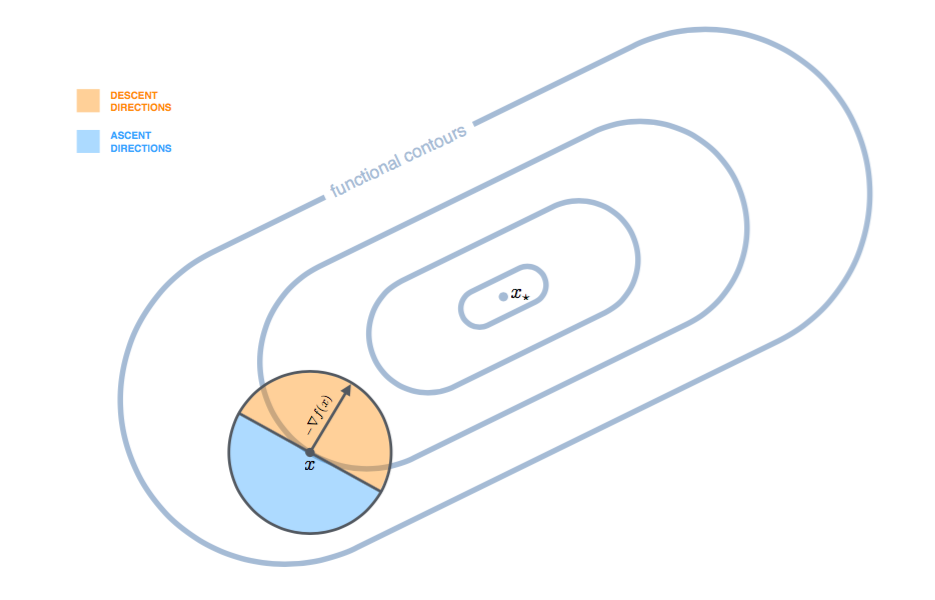
\includegraphics[width=0.8\textwidth]{descent_direction.png}
    \caption{Illustration of a descent direction.  $x-  \nabla f(x)$ is a decreasing step,
      while   $x - \delta \nabla f(x)$ goes too far and makes the result worse.}
    \label{fig:desc_dir}
  \end{figure}
  
  \autoref{fig:desc_dir} shows an example of descent directions.
  
\textbf{\textit{Lemma:}} Let $f$ be a continuously differentiable function over $\RR^n$, and let $x \in \RR^n$. Suppose that $d \neq 0 \in \RR^n$ is a descent direction of $f$ at $x$. Then there exists an $\epsilon > 0$ such that
  \begin{equation*}
      f(x + td) - f(x) < 0,
  \end{equation*}
    for all $t \in [0,\epsilon]$
    
\textbf{\textit{Proof:}} We start with a Taylor expansion
    \begin{align}
    f(x +td) - f(x)  &= \biggl(f(x) + t\nabla f(x)^T d + \mathcal{O}(t\norm{d})\biggr) - f(x)
    \\ &=   \underbrace{t\nabla f(x)^T d}_{\text{known to be $< 0$}} + \mathcal{O}(t\norm{d}) < 0
    \end{align}
    
    Since
    \begin{equation*}
        \lim\limits_{t \to 0^{+}}\frac{|\mathcal{O}(t\norm{d})|}{t} = 0
    \end{equation*}
    there exists a $\Bar{t} > 0$ s.t.
    \begin{equation*}
        \frac{|\mathcal{O}(t||d||)|}{t} < |\nabla f(x)^T d|, \quad \forall t \in (0, \Bar{t}).
    \end{equation*}

%%%%%%%%%%%%%%%%%%%%%%%%%%%%%%%%%%%%%%%%%%%%%%%%%%%%%%%%%%%
% 10 exact same
\begin{question}
 Give the general form of a gradient method and show that 
  \begin{equation*} 
    d^k = -D^k \nabla f(x^k) 
  \end{equation*}
 with $D^{k}$ symmetric and positive definite is a descent
 direction. Give three different standard choices for
 descent directions based on choosing the scaling matrix $D^{k}$ and discuss their numerical performance.
 \end{question}

\paragraph{General form of gradient method} 
\begin{enumerate}
  \item Choose an initial vector \(\kth[0]{x} \in \RR^n\)
  \item Choose a descent direction \(\kth{d}\) that satisfies \(\T{\nabla f(\kth{x})} \kth{d} < 0\)
  \item Choose a positive step size \(\kth{\alpha}\)
  \item Compute the new vector as
  \begin{equation*}
    \kth[k+1]{x} = \kth{x} + \kth{\alpha} \kth{d}
  \end{equation*}
  \item Set \(k = k + 1\) and goto 2, until some termination criterion is fulfilled
\end{enumerate}

\paragraph{Descent direction}
We have
  \begin{equation*}
    \T{\nabla f(\kth{x})} \kth{d} = -\T{\nabla f(\kth{x})} \kth{D} \nabla f(\kth{x}) < 0,
  \end{equation*}
  which follows directly from the assumption of \(\kth{D}\) being positive definite (since
  \(\T{x}\kth{D}x > 0\) for all \(x\)). 
  
\paragraph{Choices for the scaling matrix $D^{k}$}
  \begin{itemize}
\item \(\kth{D} = I\): steepest descent, slow convergence if the level lines are elongated (leads to
  zig-zagging), but easy to evaluate.
\item \(\kth{D} = (\nabla^2 f(\kth{x}))^{-1}\): Newton's method, very fast convergence near minima.
  Unstable wrt. initial values (may diverge).  Requires recalculation of inverse of Hessian in
  every step~-- very expensive in large dimensions.  Hessian might also become singular.
\item \(\kth{d} = \del[1]{\pd[2]{f(\kth{x})}{(x_i)}}^{-1}\): diagonal scaling, an approximation of
  Newton's method, but usually not worth it (scales only in diagonal directions).
\item $\kth{D} = \del[1]{\nabla g(\kth{x}) \T{\nabla g(\kth{x})}}^{-1}$: Gauss-Newton method, for
  least squares problems with design function \(g\). Good performance; again calculation of inverse,
  but not of the Hessian.
\end{itemize}

%%%%%%%%%%%%%%%%%%%%%%%%%%%%%%%%%%%%%%%%%%%%%%%%%%%%%%%%%%%
% 11 exact same
\begin{question}
Prove the formula for exact line search based on a descent direction $d$ for quadratic functions of the form
\begin{equation*}
     \min_x \dfrac{1}{2} \T{x} Ax + \T{b}x + c
\end{equation*}
\end{question}

Refresh:
\begin{itemize}
    \item $\nabla f(x) = Ax + b$
    \item $\nabla^2 f(x) = A$
\end{itemize}

Exact line search problem:
\begin{equation*}
    t^*=arg\,min_{t \geq 0} f(x + td)
\end{equation*}
with $d \in \mathbb{R} $ as a descent direction that satisfies $\nabla f(x)^Td < 0 $

Define a function $g(t)=f(x+td)$
\begin{align}
    g(t) &= \frac{1}{2}(x+td)^TA(x+td) + b^T(x+td) + c\\
    &= \frac{1}{2}t^2(d^TAd) + td^T(Ax+b) + \frac{1}{2}x^TAx + b^Tx + c\\
    \frac{\partial g(t)}{\partial t} &= t(d^TAd) + d^T(Ax+b)\\
    &= t(d^TAd) + d^T\nabla f(x)
\end{align}

Explanation
\begin{enumerate}
    \item[(1)] Put $x+td$ into $f$
    \item[(2)] Multiply
    \item[(3)] Compute derivative wrt. $t$
    \item[(4)] Substitute $Ax+b$ for $\nabla f(x)$
\end{enumerate}

From the first order necessary condition of optimality $g'(t)=0$, which is also sufficient here since we minimize a quadratic function with positive definite Hessian matrix we get the closed solution:
\begin{equation*}
    t^* = -\frac{d^T\nabla f(x)}{d^TAd} = -\frac{d^T(Ax+b)}{d^TAd}
\end{equation*}

%%%%%%%%%%%%%%%%%%%%%%%%%%%%%%%%%%%%%%%%%%%%%%%%%%%%%%%%%%%
% 12 exact same
\begin{question}
Explain the Armijo step size rule and draw a figure. Prove the sufficient decrease condition and show its relation to the Armijo step size condition.
\end{question}

	\textbf{Armijo rule:}
	\begin{equation*}
     f(\kth{x}) - f(\kth{x} + \kth{t}\kth{d}) \geq - \sigma \kth{t}  \nabla f(\kth{x})^T\kth{d}, \kth{t}=s \beta^{\kth{m}}, s > 0, \beta,\sigma \in (0,1).
	\end{equation*}
	\textbf{\textit{Lemma 15.1:}} Let f be a continuously differentiable function over $\RR^n$ with L-Lipschitz continuous gradient. Then for any $x \in \RR^n$ and $t > 0$ 
	\begin{equation*}
	    f(x) - f(x + t\nabla f(x)) \geq t(1-\frac{Lt}{2})\norm{\nabla f(x)}^2.
	\end{equation*}
	
    \textbf{\textit{Proof:}} We apply the descent lemma to $x = x$ and $y = x - t\nabla f(x)$:
    \begin{equation*}
    f(x-t\nabla f(x)) \leq f(x) - t\norm{\nabla f(x)}^2 + \frac{Lt^2}{2}\norm{\nabla f(x)}^2 = f(x) - t\biggl(1 - \frac{Lt}{2}\biggr)\norm{\nabla f(x)}^2.
	\end{equation*}
    
    \textbf{\textit{Backtracking:}} From the Armijo rule we know that
    \begin{equation*}
     f(\kth{x}) - f(\kth{x} - \kth{t}\nabla f(\kth{x})) \geq  \sigma \kth{t}  \norm{\nabla f(\kth{x})}^2, \kth{t}=s \beta^{\kth{m}}, s > 0, \beta,\sigma \in (0,1).
	\end{equation*}
	where $\kth{d}$ is such that $\nabla f(\kth{x})^T\kth{d}\leq0$. 
	
	We have to consider two cases:
	\begin{enumerate}[I:]
	\item $\kth{t} = s$ and hence the sufficient decrease condition is valid with parameter $\sigma s$.
	\item $\kth{t}$ has been determined by the backtracking procedure. This means that $\kth{\widetilde{t}} = \frac{\kth{t}}{\beta}$ which was not accepted and hence
	
	\end{enumerate}
	\begin{equation*}
     f(\kth{x}) - f(\kth{x} - \frac{\kth{t}}{\beta}\nabla f(\kth{x})) < \sigma \frac{\kth{t}}{\beta} \norm{\nabla f(\kth{x}}^2
	\end{equation*}
    
    From the sufficient decrease lemma, we also have that (choosing $x = \kth{x} , t = \frac{\kth{t}}{\beta}$)
    
    \begin{equation*}
     f(\kth{x}) - f(\kth{x} - \frac{\kth{t}}{\beta}\nabla f(\kth{x})) \geq  \frac{\kth{t}}{\beta}\biggl(1 - \frac{L\kth{t}}{2\beta}\biggr)\norm{\nabla f(\kth{x})}^2.
	\end{equation*}
	
	Combining both inequalities, we obtain
	
	\begin{align*}
     \sigma \frac{\kth{t}}{\beta} \norm{\nabla f(\kth{x})}^2 >& f(\kth{x}) - f(\kth{x} - \frac{\kth{t}}{\beta} \nabla f(\kth{x})) &\geq \frac{\kth{t}}{\beta} \biggl(1 - \frac{L\kth{t}}{2\beta} \biggr) \norm{\nabla f(\kth{x})}^2 &\\
      \sigma \frac{\kth{t}}{\beta} \norm{\nabla f(\kth{x})}^2 >&&  \frac{\kth{t}}{\beta}\biggl(1 - \frac{L\kth{t}}{2\beta}\biggr)\norm{\nabla f(\kth{x})}^2 &\\ 
      \sigma >&& \biggl(1 - \frac{L\kth{t}}{2\beta}\biggr)& 
	\end{align*}
	
	\begin{equation*} 
     1 - \frac{L\kth{t}}{2\beta} < \sigma \implies \kth{t} > \frac{2(1-\sigma)\beta}{L}.
	\end{equation*}
    
    In summary, we obtain for the step size $\kth{t} \geq min\{s,\frac{2(1-\sigma)\beta}{L}\}$ and hence
    
    \begin{equation*}
      f(\kth{x}) - f(\kth{x} - \kth{t}\nabla f(\kth{x})) \geq \sigma min\{s,\frac{2(1- \sigma) \beta}{L}\}\norm{\nabla f(\kth{x})}^2.
	\end{equation*}
	

    \begin{figure}[H]
      \centering
      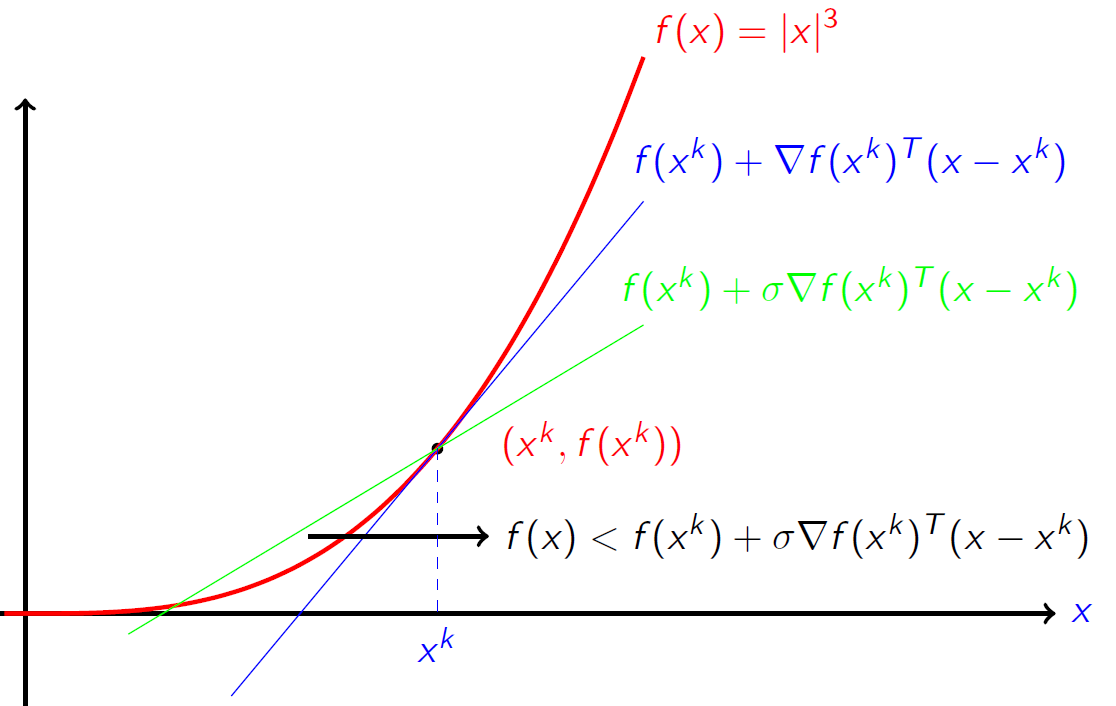
\includegraphics[width=0.8\textwidth]{armijo_rule_new.png}
      \caption{Graphical representation of the idea of the Armijo rule.  The x-axis shows $x$,
        the y-axis $f(x)$. The lines in blue and green show the different descent vector depending on the step size from the armijo rule. The green line decreases the function more than the blue line.\label{fig:armijo}}
    \end{figure}


%%%%%%%%%%%%%%%%%%%%%%%%%%%%%%%%%%%%%%%%%%%%%%%%%%%%%%%%%%%
% 13 exact same
\begin{question}
What is the "zig-zag" effect? Prove that the differences of successive iterates are orthogonal to each other when using an exact line search.
\end{question}

We proof that the steepest descent method with exact line search creates a
sequence of search directions, which are orthogonal to each other. This behavior is known
under the name ''zig-zag'' effect.

\textit{Lemma 11.1}: Let $f$ be a continuously differentiable function over $\RR^n$ and let $\{x^k\}_{k \ge0}$ be the sequence generated by the gradient method with exact line search for minimizing $f$. Then for $k \ge 0$ one has 
$$( x^{k+2} - x^{k+1})^T( x^{k+1} - x^{k}) = 0$$ 

\textit{Proof}: By the definition of the gradient method using steepest descent,
	$$x^{k+1} = x^{k}-t^{k}\nabla f(x^{k})$$
	From this follows that
    \begin{align*}
	 x^{k+1} - x^{k}&= -t^k \nabla f(x^{k})\\
	 x^{k+2} - x^{k+1} &= -t^{k+1} \nabla f(x^{k+1})
    \end{align*}
	Hence, we see that the condition $( x^{k+2} - x^{k+1})^T( x^{k+1} - x^{k}) = 0$ is equivalent to $\nabla f(x^{k})^T \nabla f(x^{k+1}) = 0$
	
	Since we are using exact line search, we have
	$$ t^{k} \in arg \min_{t \ge 0} \Big \{
	g(t) = f(x^{k}-t^{k} \nabla f(x^{k})) \Big \}$$
	
	From the necessary optimality condition $g^{'}(t^{k}) = 0$, it follows that
	$$ \nabla f(x^{k})^T \nabla f(\underbrace{x^{k}- t^{k}\nabla f(x^{k})}_{x^{k+1}}) = 0, $$
	and therefore $\nabla f(x^{k})^T \nabla f(x^{k+1}) = 0$.
	\begin{flushright}
		$\square$
	\end{flushright}
%%%%%%%%%%%%%%%%%%%%%%%%%%%%%%%%%%%%%%%%%%%%%%%%%%%%%%%%%%%
% 14 exact same
\begin{question}
What is the rate of convergence of the gradient method for quadratic functions when using exact line search. What is the condition number?
\end{question}

\textit{Theorem 6} Let $f(x) = \frac{1}{2}x^TAx$ be a quadratic function, where A is a
symmetric and positive definite matrix where $m = \lambda_{min}(A) > 0$ and $M = \lambda_{max}(A) > 0$ denote the smallest and largest
eigenvalues of A. Then the gradient method with step size $\kth{t} = \frac{2}{m+M}$ achieves the following linear convergence rate:
$$ \frac{\norm{\kth[k+1]{x}}}{\norm{\kth{x}}} \leq \frac{M-m}{M+m} \in (0,1) $$

\textit{Proof.} The gradient method takes the following form:
$$ \kth[k+1]{x} = \kth{x} - \kth{t}\nabla f(\kth{x}) = (I-\kth{t}A)(\kth{x})$$
and we have
$$\norm{\kth[k+1]{x}}^2 = \norm{(I-\kth{t}A)\kth{x}}^2$$
From the fundamental property of norms $\norm{Ax}^2_2 \leq \norm{A}^2_{2,2}\norm{x}^2_2$, we obtain the estimate
\begin{equation}
  \norm{\kth[k+1]{x}}^2 = \norm{(I-\kth{t}A)\kth{x}}^2 \leq \lambda_{max}\biggl((I-\kth{t}A)^2\biggr)\norm{\kth{x}}^2
  \label{eq:eigenvalue_norm}
\end{equation}

Let us investigate the eigenvalues of the matrix $(I-\kth{t}A)^2$. From the spectral decomposition
theorem $A = U D U^T$, where D is a diagonal matrix, having the eigenvalues of A on its diagonal and U is a unitary matrix i.e. $UU^T = U^TU = I$, we have
\begin{align*}
  (I-\kth{t}A)^2 &= (I-\kth{t}A)(I-\kth{t}A) \\
                 &= (UU^T-\kth{t}UDU^T)(UU^T-\kth{t}UDU^T) \\
                 &= U(I-\kth{t}D)U^TU(I-\kth{t}D)U^T \\
                 &= U(I-\kth{t}D)^2U^T
\end{align*}

From this we see that the eigenvalues of the matrix $(I-\kth{t}A)^2$ are given by the values $(I-\kth{t}\lambda_i(A))^2$,
$i = 1...n$. Since this expression is a convex function in $\lambda_i(A)$, the inequality (\ref{eq:eigenvalue_norm}) reduces to
$$\norm{\kth[k+1]{x}}^2 \leq max\bigl\{(1-\kth{t}m)^2, (1-\kth{t}M)^2\bigr\}\norm{\kth{x}}^2.$$
Taking square roots on both sides, we obtain
$$\norm{\kth[k+1]{x}} \leq max\biggl\{\abs{1-\kth{t}m}, \abs{1-\kth{t}M}\biggr\}\norm{\kth{x}}.$$

Since we are interested in the convergence rate of the gradient descent method, we rearrange the above inequality as
$$\frac{\norm{\kth[k+1]{x}}}{\norm{\kth{x}}} \leq max\biggl\{\abs{1-\kth{t}m}, \abs{1-\kth{t}M}\biggr\}.$$

The value $\frac{\norm{\kth[k+1]{x}}}{\norm{\kth{x}}} = \frac{\norm{\kth[k+1]{x}-x^*}}{\norm{\kth{x}-x^*}}$
determines how much the error is shrunk from one iteration to the
next. This error measure is also called a linear convergence rate. To obtain the
fastest decrease, we still have a degree of freedom, which is the step size $\kth{t}$. Indeed, the fastest
decrease is obtained by minimizing the right hand side with respect to $\kth{t}$.

Minimizing the right hand side amounts to minimizing the maximum of two absolute functions.
From \autoref{fig:intersection}, one can easily see that the
minimum value is obtained, where the line $-(1-\kth{t}M)$ intersects with the line $1-\kth{t}m$. From this we obtain that
$$\kth{t} = \frac{2}{m+M}.$$
Substituting this value for $\kth{t}$ back into the function $\abs{1-\kth{t}m}$, or $\abs{1-\kth{t}M}$, we obtain the
convergence rate
$$ \frac{\norm{\kth[k+1]{x}}}{\norm{\kth{x}}} \leq \frac{M-m}{M+m} \in (0,1).$$

	\begin{flushright}
		$\square$
	\end{flushright}
	
  \begin{figure}[htb]
    \centering
    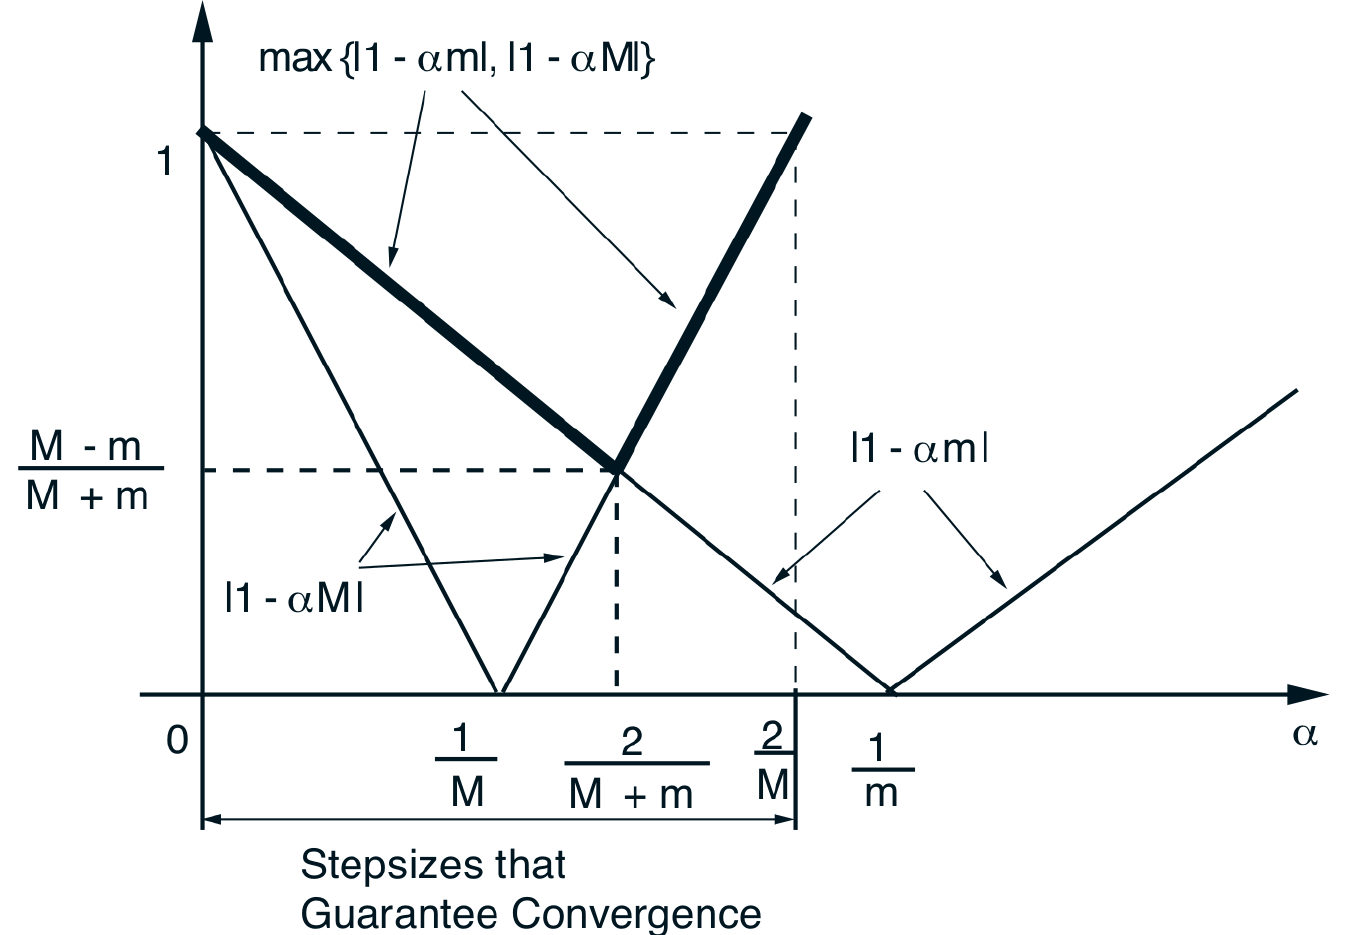
\includegraphics[width=0.8\textwidth]{convergence_intersection.png}
    \caption{\label{fig:intersection}}
  \end{figure}
  
\paragraph{Condition Number:} Let $A$ be an $n\times n$ positive definite matrix. Then, the condition
number of $A$ is defined by
$$ \kappa(A) = \frac{\lambda_{max}(A)}{\lambda_{min}(A)}.$$

 The higher the condition number of an optimization problem, the more difficult it is to solve.

%%%%%%%%%%%%%%%%%%%%%%%%%%%%%%%%%%%%%%%%%%%%%%%%%%%%%%%%%%%
% 15 Patrick
\begin{question}
What is a Lipschitz continuous gradient and show how it is related to the norm of the Hessian matrix? What is the Lipschitz constant of the gradient of a linear least squares problem of the form
\begin{equation*}
     \min_x \frac{1}{2} \norm{Ax-b}^2
\end{equation*}
\end{question}
We consider the class of unconstrained optimization problems 
\begin{equation*}
\min_{x \in \mathbb{R}^n} f(x).
\end{equation*}
A gradient $\nabla f$ is Lipschitz continuous, if there exists a $L\geq 0$ such that
\begin{equation*}
     \norm{\nabla f(x) - \nabla f(y)}_2 \leq L\norm{x-y}_2,
\end{equation*}
for any $x,y\in\mathbb{R}^n$.\\
Let $f$ be a twice continuously differentiable function over $\mathbb{R}^n$. Then the following properties are equivalent:
\begin{enumerate}[(1)]
    \item $\norm{\nabla f(x) - \nabla f(y)}_2 \leq L\norm{x-y}_2,$ for any $x,y \in \mathbb{R}^n$
    \item $\norm{\nabla^2 f(x)}_2 \leq L$ for any $x \in \mathbb{R}^n$
\end{enumerate}
\textbf{Proof:} $(1) \implies (2)$ By the fundamental theroem of calculus, one has for any $d \in \mathbb{R}^n$ and $\alpha > 0$: 
\begin{align*}
     \nabla f(x + \alpha d)= \nabla f(x) + \int_{0}^{\alpha} (\nabla^2 f(x + td)\cdot d)dt.
\end{align*}
Thus
\begin{align*}
 \norm{\int_{0}^{\alpha} (\nabla^2 f(x + td)dt \cdot d)} = \norm{\nabla f(x + \alpha d) - \nabla f(x)} \leq L \alpha \norm{d}
\end{align*}
Dividing both sides by alpha,
\begin{align*}
 \norm{\frac{1}{\alpha}\int_{0}^{\alpha} (\nabla^2 f(x + td)dt \cdot d)}  \leq L  \norm{d}
\end{align*}
By the continuity of the Hessian,
\begin{align*}
 \lim_{\alpha \implies 0^+} \frac{1}{\alpha}\int_{0}^{\alpha} \nabla^2 f(x + td)dt = \nabla^2 f(x),
\end{align*}
from which it follows that $\norm{\nabla^2 f(x) \cdot d} \leq L\norm{d}$. Finally dividing both sides by $\norm{d}$ and taking the supremum with respect to $d$ yields
\begin{align*}
 \sup_{d \neq 0} \frac{\norm{\nabla^2 f(x) \cdot d}}{\norm{d}} \leq L
\end{align*}
The left hand side is exactly the definition of the operator norm and hence we obtain 
\begin{align*}
  \norm{\nabla^2 f(x)} \leq L
\end{align*}

\textbf{Linear least squares problem:} $f(x) = \frac{1}{2} \norm{Ax - b}^2 = \frac{1}{2}x^T A^T Ax -b^TAx + \frac{1}{2} \norm{b}^2$, $\nabla f(x) = A^TAx - A^Tb$ have a Lipschitz continuous gradient with $L=\norm{A^TA}_2 = \sigma_{max}(A^TA)$, since
\begin{align*}
    \norm{(A^TAx-A^Tb) - (A^TAy - A^Tb)}_2 &\leq L \norm{x-y}_2\\
    \norm{A^TA(x-y)}_2 \leq \norm{A^TA}_2\norm{x-y}_2 &\stackrel{!}{=} L \norm{x-y}_2\\
    \norm{\T{A}A}_2 &\stackrel{!}{=} L
\end{align*}
%%%%%%%%%%%%%%%%%%%%%%%%%%%%%%%%%%%%%%%%%%%%%%%%%%%%%%%%%%%
% 16 Patrick
\begin{question}
Prove the descent lemma for a differentiable function $f$ with Lipschitz-continuous gradient. Interpret the inequality of the descent lemma in terms of an upper bound to the function $f$. Use the descent lemma to also prove the sufficient decrease lemma.
\end{question}

One of the most important results for functions with Lipschitz continuous gradients is that they can be globally bounded from above by quadratic functions scaled by the Lipschitz constant.
This result is known as the descent lemma and plays a major role in the convergence proof of gradient methods.


\textbf{Descent lemma:}\\
\textbf{Theorem:} Let $f$ be a continuously differentiable function over $\RR^n$ with L-Lipschitz continuous gradient. Then, for any $x, y \in \RR^n$:
\begin{equation*}
    f(y) \leq f(x) + \nabla f(x)^T(y-x)+\frac{L}{2} ||y-x||^2
\end{equation*}

\textbf{Proof:}\\
Let $g(t) = f(x + t(y-x))$, so that $g(0)=f(x)$ and $g(1)=f(y)$.
Then
\begin{align}
    f(y) &= f(x) + f(y) - f(x)\\
         &= f(x) + g(1) - g(0)\\
         &= f(x) + \int_{0}^{1} g'(t) \text{d}t\\
         &= f(x) + \int_{0}^{1} \nabla f(x + t(y-x))^T(y-x)\text{d}t\\
         &= f(x) + \int_{0}^{1} \langle \nabla f(x) + \nabla f(x + t(y-x)) - \nabla f(x), y-x \rangle \text{d}t\\
         &= f(x) + \int_{0}^{1} \langle \nabla f(x), y-x \rangle \text{d}t + \int_{0}^{1} \langle \nabla f(x + t(y-x)) - \nabla f(x), y-x \rangle \text{d}t\\
         &\leq f(x) + \langle \nabla f(x), y-x \rangle + \int_{0}^{1} || \nabla f(x + t(y-x)) - \nabla f(x) || \cdot ||y-x|| \text{d}t\\
         &\leq f(x) + \langle \nabla f(x),y-x \rangle + ||y-x|| \int_{0}^{1} Lt||y-x|| \text{d}t\\
         &= f(x) + \langle \nabla f(x) ,y-x \rangle + \frac{L}{2} ||y-x||^2\\
         &= f(x) + \nabla f(x)^T (y-x) + \frac{L}{2} ||y-x||^2
\end{align}

\textbf{Explanation of steps:}
\begin{itemize}
    \item (1): Simple expansion
    \item (2): Rewrite to $g(t)$ functions
    \item (3): Rewrite to integral from 0 to 1 (fundamental theorem of calculus)
    \item (4): Derivation $\frac{\partial}{\partial t}$
    \item (5): Rewrite to inner product and expand with $\nabla f(x)$
    \item (6): Separate into 2 separate integrals preserving the inner product inside
    \item (7): Left integral computed, Application of the Cauchy-Schwarz Theorem: $|\langle x,y \rangle| \leq ||x|| \cdot ||y||$ 
    \item (8): Follows from Lipschitz continuity of the gradient:
    \begin{align*}
        ||\nabla f(x+t(y-x)) - \nabla f(x)|| &\leq L||x+t(y-x) - x||\\
        &= L||t(y-x)||\\
        &= Lt||y-x||
    \end{align*}
    \item (9): Integrate
    \item (10): Rewrite inner product
\end{itemize}

\textbf{Sufficient Decrease Lemma:}\\
Let $f$ be a continuously differentiable function over $ \mathbb{R}^n$ with  L-Lipschitz continuous gradient. Then for any $x\in \mathbb{R}^n$ and $t>0$
\begin{equation*}
	    f(x) - f(x - t\nabla f(x)) \geq t(1-\frac{Lt}{2})\norm{\nabla f(x)}^2.
\end{equation*}
\textbf{\textit{Proof:}} We apply the descent lemma to $x = x$ and $y = x - t\nabla f(x)$:
    \begin{equation*}
    f(x-t\nabla f(x)) \leq f(x) - t\norm{\nabla f(x)}^2 + \frac{Lt^2}{2}\norm{\nabla f(x)}^2 = f(x) - t\biggl(1 - \frac{Lt}{2}\biggr)\norm{\nabla f(x)}^2.
	\end{equation*}
	
% Let us now analyze the outcome of the sufficient decrease lemma for different choices of the
% step size:
% \begin{enumerate}
%     \item \textbf{\textit{Constant step size:}} In case of a constant step size, it is easy to see that we have $t(1-\frac{Lt}{2}) > 0$, (such that the function values are decreasing in each step) as long as $t \in (0,2/L)$. Maximal descent is achieved by maximizing the factor $t(1-\frac{Lt}{2})$ with respect to $t$ . Clearly the maximum is attained for $t = \frac{1}{L}$. In this case the decrease of the function
% values is given by
%     \begin{equation*}
%      f(\kth{x}) -f(x^{(k+1)}) = f(\kth{x})-f(\kth{x}- \frac{1}{L} \nabla f(x)) \geq \frac{1}{2L} \norm{\nabla f(x)}^2.
% 	\end{equation*}
%      \item \textbf{\textit{Exact line search:}}In the exact line search, the step size $t^k$ is determined via
%      \begin{equation*}
%      \kth{t} = \argmin_t f(\kth{x} - t\nabla f(\kth{x})).
% 	\end{equation*}
% 	From the optimality of $t^k$ we directly obtain that
% 	 \begin{equation*}
%       f(\kth{x}-\kth{t} \nabla f(\kth{x})) \leq f(\kth{x} - \frac{1}{L} \nabla f(\kth{x})).
% 	\end{equation*}
% 	hence
% 	\begin{equation*}
% 	    f(\kth{x}) -f(x^{(k+1)}) \geq f(\kth{x}) - f(\kth{x} - \frac{1}{L} \nabla f(\kth{x})) \geq \frac{1}{2L} \norm{\nabla f(x)}^2.
% 	\end{equation*}
        
%      \item  \textbf{\textit{Backtracking:}} From the Armijo rule we know that
%     \begin{equation*}
%      f(\kth{x}) - f(\kth{x} - \kth{t}\nabla f(\kth{x})) \geq \sigma \kth{t} \norm{\nabla f(\kth{x})}^2, \kth{t}=s \beta^{\kth{m}}, s > 0, \beta,\sigma \in (0,1).
% 	\end{equation*}
	
% 	We have to consider two cases:
% 	\begin{enumerate}[I:]
% 	\item $\kth{t} = s$ and hence the sufficient decrease condition is valid with parameter $\sigma s$.
% 	\item $\kth{t}$ has been determined by the backtracking procedure. This means that $\kth{\widetilde{t}} = \frac{\kth{t}}{\beta}$ which was not accepted and hence
	
% 	\end{enumerate}
% 	\begin{equation*}
%      f(\kth{x}) - f(\kth{x} - \frac{\kth{t}}{\beta}\nabla f(\kth{x})) < \sigma \frac{\kth{t}}{\beta} \norm{\nabla f(\kth{x}}^2
% 	\end{equation*}
    
%     From the sufficient decrease lemma, we also have that (choosing $x = \kth{x} , t = \frac{\kth{t}}{\beta}$)
    
%     \begin{equation*}
%      f(\kth{x}) - f(\kth{x} - \frac{\kth{t}}{\beta}\nabla f(\kth{x})) \geq  \frac{\kth{t}}{\beta}\biggl(1 - \frac{L\kth{t}}{2\beta}\biggr)\norm{\nabla f(\kth{x})}^2.
% 	\end{equation*}
	
% 	Combining both inequalities, we obtain
	
% 	\begin{align*}
%      \sigma \frac{\kth{t}}{\beta} \norm{\nabla f(\kth{x})}^2 >& f(\kth{x}) - f(\kth{x} - \frac{\kth{t}}{\beta} \nabla f(\kth{x})) &\geq \frac{\kth{t}}{\beta} \biggl(1 - \frac{L\kth{t}}{2\beta} \biggr) \norm{\nabla f(\kth{x})}^2 &\\
%       \sigma \frac{\kth{t}}{\beta} \norm{\nabla f(\kth{x}}^2 >&&  \frac{\kth{t}}{\beta}\biggl(1 - \frac{L\kth{t}}{2\beta}\biggr)\norm{\nabla f(\kth{x})}^2 &\\ 
%       \sigma >&& \biggl(1 - \frac{L\kth{t}}{2\beta}\biggr)& 
% 	\end{align*}
	
% 	\begin{equation*} 
%      1 - \frac{L\kth{t}}{2\beta} < \sigma \implies \kth{t} > \frac{2(1-\sigma)\beta}{L}.
% 	\end{equation*}
    
%     In summary, we obtain for the step size $\kth{t} \geq min\{s,\frac{2(1-\sigma)\beta}{L}\}$ and hence
    
%     \begin{equation*}
%       f(\kth{x}) - f(\kth{x} - \kth{t}\nabla f(\kth{x})) \geq \sigma min\{s,\frac{2(1- \sigma) \beta}{L}\}\norm{\nabla f(\kth{x})}^2.
% 	\end{equation*}
% \end{enumerate}

%%%%%%%%%%%%%%%%%%%%%%%%%%%%%%%%%%%%%%%%%%%%%%%%%%%%%%%%%%%
% 17 exact same
\begin{question}
Give the general form of non-linear least-squares problems. Show how the Gauss-Newton method is obtained from performing a first-order Taylor approximation. What is the Levenberg-Marquardt method?
\end{question}

\begin{itemize}
    \item General form:
        \begin{equation*}
          f(x) = \frac{1}{2} \enVert[1]{g(x)}^2 = \frac{1}{2} \sum_i \enVert[1]{g_i(x)}^2,
        \end{equation*}
        Often, a least squares problem is a model fitting problem, where
        \begin{equation*}
          g_i(\theta) = h(x_i, \theta) - \hat{y}_i.
        \end{equation*}
    For the problem to be non-linear, the hypothesis $h(x_i, \theta)$ has to be non linear.
    
    \item The first-order approximation of g around $\kth{x}$:
        \begin{equation*}
         \widetilde{g}(x,\kth{x})=g(\kth{x}) + \nabla \T{g(\kth{x})} (x-\kth{x}),
        \end{equation*}
        which yields
        \begin{align*}
            \widetilde{f}(x,\kth{x}) &= \dfrac{1}{2} \norm{\widetilde{g}(x,\kth{x})}^2 
            \\ &=   \dfrac{1}{2} \norm{ g(\kth{x}) + \nabla \T{g(\kth{x})}(x-\kth{x})}^2,
        \end{align*}
        
        Computing the gradient of the last expression with respect to $x$ and setting it to zero yields
        
        \begin{align*}
            0 &\overset{!}{=}  \nabla g(\kth{x})\biggl(g(\kth{x}) +
                 \nabla \T{g(\kth{x})} (\kth[k+1]{x} - \kth{x})\biggr)
            \\ &= \nabla g(\kth{x})g(\kth{x}) +
                 \nabla g(\kth{x})\nabla \T{g(\kth{x})} (\kth[k+1]{x} - \kth{x})
            \\ \kth[k+1]{x} &= \kth{x} - \bigl ( \nabla g(\kth{x} ) \nabla \T{g(\kth{x})})^{-1}\nabla g(\kth{x})g(\kth{x}),
        \end{align*}
        assuming that $\nabla g(\kth{x})\nabla \T{g(\kth{x})}$ is invertible. If $g$ is linear, this method reduces
    to the Moore-Penrose pseudoinverse and solves the problem in one step.
    \item Levenberg-Marquardt Method: 
        To ensure that $\nabla g(\kth{x}) \nabla \T{g(\kth{x})}$ is invertible, and the descent direction is actually gradient related, one can use a modified iteration scheme

        \begin{equation*}
            \kth[k+1]{x} = \kth{x} - \kth{\alpha}(\nabla g( \kth{x}) \T{\nabla g( \kth{x})} + \kth{\delta}I)^{-1} \nabla g(\kth{x})g(\kth{x}),
        \end{equation*}
        where $\kth{\alpha}$ can be chosen by the Armijo rule, and $ \kth{\delta} > 0$ large enough.
\end{itemize}

%%%%%%%%%%%%%%%%%%%%%%%%%%%%%%%%%%%%%%%%%%%%%%%%%%%%%%%%%%%
% 18 exact same
\begin{question}
Explain the Kalman filter and show its relation to incremental Gauss-Newton methods. What are its applications?
\end{question}

The Kalman filter is an incremental Gauss-Newton method.

If a least-squares model (i.e. the functions \(g_i\)) is linear, one Gauss-Newton iteration would be
enough to find the optimal solution (this amounts to the analytical solution using the Moore-Penrose
pseudoinverse).  However, we can develop an incremental method for this, avoiding the matrix
inversion, and instead using one sample at a time.

Concretely, for \(g_i(x) = z_i - C_i x\), we have a step method
\begin{align*}
  \xi_i &= \xi_{i-1} + H_i^{-1}\T{C_i}(z_i - C_i \xi_{i-1}), \quad\text{with} \\
  H_i &= \lambda H_{i-1} + \T{C_i}C_i, \quad H_0 = 0 \text{ and } \xi_0 \text{ arbitrary}.
\end{align*}

which iteratively generates the incrementally growing least squares estimate
$$ \xi_i \in \argmin_x \sum_{j=1} ^{i}\lambda^{i-j}\norm{z_j-C_jx}^2, \quad i=1,\dots,m$$

\paragraph{Derivation from Gauss-Newton method}
The problem of the first block is given by 

$$ \xi_1 = \argmin_x \frac{1}{2}\norm{z_1-C_1x}^2.$$
Its optimal solution using Gauss-Newton method is given by
$$\xi_1 = (C_1^TC_1)^{-1}C_1^Tz_1.$$

Therefore, for any $\xi_0$ by just expanding with
\begin{equation*}
    \underbrace{\xi_0 - \underbrace{(C_1^TC_1)^{-1}C_1^TC_1}_{= I}\xi_0}_{= 0}
\end{equation*}
we get
\begin{align*}
  \xi_1 &= \xi_0 - (C_1^TC_1)^{-1}C_1^TC_1\xi_0+(C_1^TC_1)^{-1}C_1^Tz_1 \\
        &= \xi_0 + (C_1^TC_1)^{-1}C_1^T (z_1-C_1\xi_0).
\end{align*}

The problem after arrival of the second problem is given by
$$ \xi_2 = \argmin_x \frac{1}{2}(\norm{z_1-C_1x}^2+\norm{z_2-C_2x}^2)$$
and its optimal solution is given by
$$\xi_2 = (C_1^TC_1+C_2^TC_2)^{-1}(C_1^Tz_1+C_2^Tz_2).$$

Hence
\begin{align}
  (C_1^TC_1+C_2^TC_2)\xi_2 &= C_1^Tz_1+C_2^Tz_2 \\
                           &= C_1^TC_1\xi_1+C_2^Tz_2 \\
                           &= C_1^TC_1 \xi_1 + C_2^TC_2 \xi_1 - C_2^TC_2\xi_1 + C_2^Tz_2\\
                           &= (C_1^TC_1+C_2^TC_2)\xi_1-C_2^TC_2\xi_1+C_2^Tz_2
\end{align}
$$\implies \xi_2 = \xi_1 + (C_1^TC_1+C_2^TC_2)^{-1}C_2^T(z_2-C_2\xi_1).$$
$$\implies \xi_2 = \xi_1 + H_2^{-1}C_2^T(z_2-C_2\xi_1).$$

$\lambda$ is set to 1 in this proof.

Explanation:
\begin{itemize}
    \item ad (2): Substitute $C_1^Tz_1$ with $C_1^T C_1 \xi_1$ (converted from the optimal solution of $\xi_1$).
    \item ad (3): Expand with $+ C^T_2 C_2 \xi_1 - C^T_2 C_2 \xi_1$
    \item ad (4): Factor out $\xi_1$
\end{itemize}

Further steps are obtainted via induction.

%%%%%%%%%%%%%%%%%%%%%%%%%%%%%%%%%%%%%%%%%%%%%%%%%%%%%%%%%%%
% 19 exact same
\begin{question}
Show that the plain form of Newton's method can be derived from a second order Taylor approximation of the objective function. Show that Newton's method is invariant with respect to affine scalings.
\end{question}

\textbf{Derivation of Newton's method from second order Taylor approximation:}\\
Start with Taylor expansion of the second order.
\begin{equation*}
    f^{(k)}(x) = f(x^{(k)}) + \nabla f(x^{(k)})^T(x-x^{(k)}) + \frac{1}{2}(x-x^{(k)})^T \nabla^2 f(x^{(k)})(x-x^{(k)})
\end{equation*}

Compute derivative wrt. $x$ and set to $0$.
\begin{equation*}
    \frac{\partial f^{(k)}(x)}{\partial x}=\nabla f(x^{(k)}) + \nabla^2 f(x^{(k)})(x-x^{(k)}) \overset{!}{=} 0
\end{equation*}

Substitute $x^{(k+1)}$ for $x$ and solve for to get the new iterate $x^{(k+1)}$.
\begin{equation*}
    x^{(k+1)} = x^{(k)} - \nabla^2 f(x^{(k)})^{-1} \nabla f(x^{(k)})
\end{equation*}

\textbf{Affine scaling invariance:}\\
The goal is to change the variables $x$ to a scaled version $x=Sy$ and then to minimize the function $f(Sy)$.
\begin{align*}
    \frac{\partial f(Sy)}{\partial y} &= S^T \nabla f(Sy)\\
    \frac{\partial^2 f(Sy)}{\partial^2 y} &= S^T \nabla^2 f(Sy)S
\end{align*}

Second order Taylor expansion of $f(Sy)$ around a given iteration $y^{(k)}$ is given by
\begin{equation*}
    f^{(k)}(y) = f(Sy^{(k)}) + \biggl(S^T \nabla f(Sy^{(k)})\biggr)^T(y-y^{(k)}) + \frac{1}{2}(y-y^{(k)})^T S^T \nabla^2 f(Sy^{(k)})S(y-y^{(k)})
\end{equation*}

Compute the derivative wrt. $y$ and set it to 0.
\begin{equation*}
    \frac{\partial f^{(k)}(y)}{\partial y} = S^T \nabla f(Sy^{(k)}) + S^T \nabla^2 f(Sy^{(k)})S(y-y^{(k)}) \overset{!}{=}0
\end{equation*}

Solving for $y$ results in the new iterate $y^{(k+1)}$.
\begin{align*}
    y^{(k + 1)} &= y^{(k)} - (S^T \nabla^2f(Sy^{(k)})S)^{-1} S^T \nabla f(Sy^{(k)})\\
            &= y^{(k)} - (\nabla^2f(Sy^{(k)})S)^{-1} (S^T)^{-1} S^T \nabla f(Sy^{(k)})\\
            &= y^{(k)} - S^{-1}\nabla^2f(Sy^{(k)})^{-1} (S^T)^{-1} S^T \nabla f(Sy^{(k)})\\
            &= y^{(k)} - S^{-1} \nabla^2 f(Sy^{(k)})^{-1} \nabla f(Sy^{(k)})
\end{align*}

Multiply from the left with $S$.
\begin{equation*}
    Sy^{(k+1)} = Sy^{(k)} - \nabla^2 f(Sy^{(k)})^{-1} \nabla f(Sy^{(k)})
\end{equation*}

Replacing $Sy^{(k)}$ with $x^{(k)}$ yields that the sequences $\{{x^{(k)}\}}_{{(k)} \geq 0}$ and $\{{Sy^{(k)}\}}_{{(k)} \geq 0}$ are equivalent. The result after replacing is
\begin{equation*}
    x^{(k+1)} = x^{(k)} - \nabla^2 f(x^{(k)})^{-1} \nabla f(x^{(k)}).
\end{equation*}

%%%%%%%%%%%%%%%%%%%%%%%%%%%%%%%%%%%%%%%%%%%%%%%%%%%%%%%%%%%
% 20 exact same
\begin{question}
Give the theorem of locally quadratic convergence of the pure form of Newton’s method and prove it. What can you say about the global convergence of Newton’s method?
\end{question}

\textit{Theorem}: Let $f$ be a twice continuously differentiable function defined over $\mathbb{R}^n$. Assume that $\nabla^2 f(x) \geq mI$ , for some $m > 0$ and any $x \in \mathbb{R}^n$. Moreover, assume that $\norm{\nabla^2 f(x) - \nabla^2 f(y)} \leq L\norm{x -y } $ for some $L > 0$ and any $x; y \in \mathbb{R}^n$. Let $\{\kth{x}\}_{k\geq0}$ be a sequence generated by the pure
form of Newton’s method and let $x^{*}$ be the unique minimizer of $f(x)$ over $\mathbb{R}^n $. Then for any $k \geq 0$ it holds that

\begin{equation*}
    \norm{\kth[k+1]{x} - x^{*}} \leq  \dfrac{L}{2m} \norm{\kth{x} - x^{*}}^{2}. 
\end{equation*}

Moreover, if $\norm{x^{(0)} - x^{*}} \leq \dfrac{m}{L}$, then

\begin{equation*}
    \norm{\kth{x} - x^{*}} \leq  \dfrac{2m}{L} \biggl(\dfrac{1}{2}\biggr)^{2^{k}}
\end{equation*}

\textit{Proof}: Let $x^{*}$ be the unique minimizer of $f(x)$, i.e. $\nabla f(x^{*}) = 0$. We start by making use of the
pure form of Newton’s method:

\begin{align}
    \kth[k+1]{x}  &= \kth{x}  - \nabla^2 f(\kth{x})^{-1}\nabla f(\kth{x})
    \\ \kth[k+1]{x} - x^{*} &= \kth{x}  - x^{*} - \nabla^2 f(\kth{x})^{-1}\nabla f(\kth{x}) 
    \\ &= \kth{x} - x^{*}  + \nabla^2 f(\kth{x})^{-1} ( 0 - \nabla f(\kth{x})   
    \\ &= \kth{x} - x^{*}  + \nabla^2 f(\kth{x})^{-1} ( \nabla f(x^{*}) - \nabla f(\kth{x})    
    \\ &= \kth{x} - x^{*}  + \nabla^2 f(\kth{x})^{-1} \Bigl[ \nabla f(\kth{x} + t(x^{*}-\kth{x})) \Bigr]_{t=0}^1
    \\ &= \kth{x} - x^{*}  + \nabla^2 f(\kth{x})^{-1} \int_{0}^{1} \biggl(\nabla f(\kth{x} + t(x^{*}-\kth{x}))\biggr)'dt
    \\ &= \kth{x} - x^{*}  + \nabla^2 f(\kth{x})^{-1} \int_{0}^{1} \nabla^2 f(\kth{x} + t(x^{*}-\kth{x}))^T(x^{*} - \kth{x})dt
    \\ &= -( x^{*} - \kth{x})  + \nabla^2 f(\kth{x})^{-1} \int_{0}^{1} \nabla^2 f(\kth{x} + t(x^{*}-\kth{x}))^T(x^{*} - \kth{x})dt
    \\ &= \nabla^2 f(\kth{x})^{-1}\biggl( \int_{0}^{1} \nabla^2 f(\kth{x} + t(x^{*}-\kth{x}))^T(x^{*} - \kth{x})dt - \nabla^2 f(\kth{x})^T( x^{*} - \kth{x})\biggr)
    \\ &= \nabla^2 f(\kth{x})^{-1} \int_{0}^{1} \biggl(\nabla^2 f(\kth{x} + t(x^{*}-\kth{x})) - \nabla^2  f(\kth{x})\biggr)^T(x^{*} - \kth{x})dt &
\end{align}

Explanation:
\begin{itemize}
    \item (3): Switch $+$ and $-$ and expand with zero to prepare for next step
    \item (4): Substitute 0 with $\nabla f(x^*)$
    \item (5): Rewrite into new function that has the same output depending on value of $t$ and write into interval notation
    \item (6): Rewrite into integral with derivative wrt. $t$
    \item (7): Compute derivative
    \item (8): Switch $+$ and $-$ in front
    \item (9): Factor in by multiplying with inverse of Hessian from the front
    \item (10): Combine with integral
\end{itemize}

From $\nabla^2 f(x) \geq mI$ it follows that $\nabla^2 f(x)^{-1} \leq \dfrac{1}{m}I$ and hence the operator norm $\norm{\nabla^2 f(x)^{-1}} \leq \dfrac{1}{m}$. With these estimates we obtain (using the fact that $\norm{Ax}\leq \norm{A}\norm{x}$)

\begin{equation*}\begin{aligned}
    \norm{\kth[k+1]{x}-x^{*}} &\leq \norm{\nabla^2 f(\kth{x})^{-1}} \norm{\int_{0}^{1} \biggl(\nabla^2 f(\kth{x} + t(x^{*}-\kth{x})) - \nabla^2 f(\kth{x})\biggr)^T(x^{*} - \kth{x})dt}
    \\ &\leq \dfrac{1}{m} \norm{\int_{0}^{1} \biggl(\nabla^2 f(\kth{x} + t(x^{*}-\kth{x})) - \nabla^2 f(\kth{x})\biggr)^T(x^{*} - \kth{x})dt}
    \\ &\leq \dfrac{1}{m} \int_{0}^{1} \norm{\nabla^2 f(\kth{x} + t(x^{*}-\kth{x})) - \nabla^2 f(\kth{x})}\norm{x^{*} - \kth{x}}dt,
\end{aligned}\end{equation*}
    because of the assumption that $\norm{\nabla^2 f(x) - \nabla^2 f(y)} \leq L\norm{x -y } $ for some $L > 0$
\begin{align*}
    \\ &\leq \dfrac{1}{m}  \int_{0}^{1} L\norm{\kth{x} + t(x^{*}-\kth{x}) - \kth{x}} \norm{x^{*}-\kth{x}}dt
    \\ &\leq \dfrac{1}{m}  \int_{0}^{1} L\norm{ t(x^{*}-\kth{x})} \norm{x^{*}-\kth{x}}dt
    \\ &= \dfrac{1}{m}  \int_{0}^{1} t L \norm{x^{*}-\kth{x}}^2dt
    \\ &= \dfrac{L}{m} \norm{x^{*}-\kth{x}}^2  \int_{0}^{1} t dt
    \\ &=  \dfrac{L}{2m}  \norm{x^{*}-\kth{x}}^2.
\end{align*}

For $k = 0$ we have assumed that $\norm{x^{(0)} - x^*} \leq \frac{m}{L}=\frac{2m}{L}(\frac{1}{2})^{2^0}$ , which serves as the base case for
our induction. Hence, for our induction hypothesis we assume that

\begin{align*}
    \norm{\kth{x} -x^*} \leq \frac{2m}{L}\biggl(\frac{1}{2}\biggr)^{2^k},
\end{align*}

holds for any k. In our induction step, we then obtain

\begin{equation*}\begin{aligned}
    \norm{\kth[k+1]{x} -x^*} \leq \frac{L}{2m} \norm{\kth{x}-x^*}^2 \leq \frac{L}{2m} \biggl(\frac{2m}{L} \biggl(\frac{1}{2}\biggr)^{2^k}\biggr)^2=\frac{2m}{L}\biggl(\frac{1}{2}\biggr)^{2^{k+1}}.
\end{aligned}\end{equation*}

%%%%%%%%%%%%%%%%%%%%%%%%%%%%%%%%%%%%%%%%%%%%%%%%%%%%%%%%%%% 
% 21 exact same

\begin{question}
What is Q-conjugacy? Show how the Gram-Schmidt procedure can be
used to generate a set of Q-conjugate directions from a set of linearly
independent vectors.
\end{question}


	\textbf{\textit{Q-conjugacy:}}
		Given a positive definite matrix $Q$ we say that a set of nonzero vectors $\{d_1,...,d_k\}$ are Q-conjugate if
		$$ d_i^T Q d_j = 0, \quad \forall i,j : i \neq j$$
		if $\{d_1,...,d_k\}$ are Q-conjugate then they are also linear independent.
	
	\textbf{\textit{Gram-Schmidt:}}
		Let $d,\xi \in \RR^n$ be two non-zero vectors which are linearly independent. The projection of vector $\xi$ onto $d$ is computed as
		$$ proj_d(\xi) = \xi^T \frac{d}{||d||}\frac{d}{||d||} = \frac{\xi^T d}{d^Td}d$$
		
		\begin{figure}
			\centering
			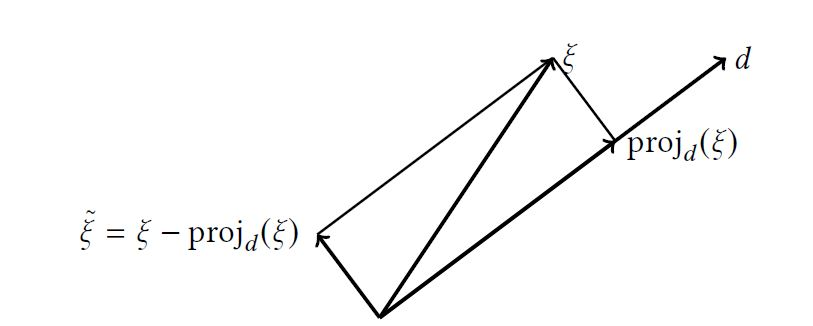
\includegraphics[width=0.5\textwidth]{figures/proj.jpg}
			\caption{Projection of the vector $\xi$ onto the vector $d$}
		\end{figure}
		
		Removing the projection of $\xi$ onto $d$ yields a vector $\tilde{\xi}$ which is orthogonal to $d$.
		$$\tilde{\xi} = \xi - proj_d(\xi)$$
		
		A simple computation shows that indeed 
		
		$$d^T \tilde{\xi} = d^{T} (\xi - proj_d(\xi)) = d^{T}(\xi - \frac{\xi^T d}{d^Td}d) = d^{T} \xi - \xi^{T}d = 0$$
		The projection can be generalized to a general metric $Q \succ 0$, by simply replacing the vector dot product $d^{T}\xi$ with $d^{T}Q\xi$ corresponding in 
		$$ proj_d^Q(\xi) = \frac{\xi^T Q d}{d^TQd}d$$
		and a vector which is $Q$-conjugate is obtained by
		$$\tilde{\xi} = \xi - proj_d^Q(\xi)$$
		Again, a simple computation shows that $d$ and $\tilde{\xi}$ are $Q$-conjugate:
		$$d^T Q \tilde{\xi} = d^{T}Q (\xi - proj_d^Q(\xi)) = d^{T}Q(\xi - \frac{\xi^T Qd}{d^TQd}d) = d^{T} Q \xi - \xi^{T} Q d = 0$$
		
		Now, given a set of linearly independent vectors $\{\xi^i\}^k_{i=0}$, we can generate pairwise $Q$-conjugate vectors $\{d^i\}^k_{i=0}$ via the\textbf{ Gram-Schmidt procedure}:
		$$ d^0 = \xi^0$$
		$$ d^{(i+1)} = \xi^{(i+1)} - \sum_{m = 0}^{i} proj_{d^m}^{Q}(\xi^{(i+1)}), \quad i = 0,...,k-1$$
%%%%%%%%%%%%%%%%%%%%%%%%%%%%%%%%%%%%%%%%%%%%%%%%%%%%%%%%%%% 

%%%%%%%%%%%%%%%%%%%%%%%%%%%%%%%%%%%%%%%%%%%%%%%%%%%%%%%%%%% 
% 22 Moritz
\begin{question}
 Write down the conjugate gradients (CG) method. What is its convergence rate and how can it be generalized to non-linear problems.

%   ---Alt---
%   Write down the conjugate gradient (CG) method and specialize the algorithm for solving a
%   least-squares problem of the form
%   \[
%     \min_x f(x) = \frac{1}{2} \T{x} Q x - \T{b} x.
%   \]
%   What is the relation to solving linear system of equations?
\end{question}

Originally, conjugate direction methods were developed to solve quadratic optimization problems of the form
\begin{equation*}
    \min_x f(x) = \frac{1}{2} \T{x} Q x - \T{b} x.
\end{equation*}
with $Q$ symmetric and positive definite.

The step scheme for the CG method is
\begin{equation*}
  \kth[k+1]{x} = \kth{x} + \kth{\alpha}\kth{d},
\end{equation*}
where $\kth{\alpha}$ is chosen by line search, and the descent directions are obtained by
orthogonalizing the gradient vectors at the successive steps, using the Gram-Schmidt procedure with
respect to the metric defined by \(Q\).

For a quadratic problem, we set
\begin{equation*}
  \kth{g} = \nabla f(\kth{x}) = Q \kth{x} - b,
\end{equation*}
and calculate the descent directions as
\begin{align*}
  \kth[0]{d} &= -\kth[0]{g}, \\
  \kth[k]{d} &= -\kth{g} + \kth{\beta}\kth[k-1]{d},
\end{align*}
where \(\kth{\beta}\) is given by
\begin{equation*}
  \kth{\beta} = \frac{||\kth{g}||^2}{||\kth[k-1]{g}||^2} = \frac{\T{(\kth{g})}\kth{g}}{\T{(\kth[k-1]{g})}\kth[k-1]{g}}.
\end{equation*}

\textit{\textbf{Convergence Rate:}}

The CG method is the optimal first order method for quadratic problems.

If $0 < l \leq Q \leq L$ is positive definite then
\begin{equation*}
    ||\kth{x} - x^*|| \leq 2 \sqrt{L/l} \left( \frac{\sqrt{L/l} - 1}{\sqrt{L/l} + 1} \right)^k ||\kth[0]{x} - x^* ||
\end{equation*}

If $0 \leq Q \leq L$ is positive semidefinite then
\begin{equation*}
    f(\kth{x}) - f(x^*) \leq \frac{L||\kth[0]{x} - x^*||^2}{2(2k + 1)^2}
\end{equation*}


\textit{\textbf{Non-linear problems:}}
For general problems of the form
\begin{equation*}
    \min_x f(x)
\end{equation*}

The only things that change are the direction $\kth{d}$ and $\kth{\beta}$:
\begin{align*}
    \kth{d} &= -\nabla f(\kth{x}) + \kth{\beta}\kth[k-1]{d}\\
    \kth{\beta} &= \frac{\nabla f(\kth{x})^T (\nabla f(\kth{x}) - \nabla f(\kth[k-1]{x}))}{\nabla f(\kth[k-1]{x})^T \nabla f(\kth[k-1]{x}) }
\end{align*}

It might be necessary to periodically restart $\kth{\beta}=0$.\\
Nothing known about the convergence rate.


%%%%%%%%%%%%%%%%%%%%%%%%%%%%%%%%%%%%%%%%%%%%%%%%%%%%%%%%%%%
%23 exact same
\begin{question}
Explain the heavy-ball algorithm and show that it is obtained from a finite differences approximation of the heavy-ball with friction dynamical system. How is it related to the CG method?
\end{question}

This is a method that uses a kind of physics related model where friction plays an important role.

We use a multi step iteration scheme:
\begin{equation*}
    x^{(k+1)} = x^{(k)} - \alpha^{(k)} \nabla f(x^{(k)}) + \beta^{(k)} (x^{(k)} - x^{(k - 1)})
\end{equation*}
Where the term $(x^{(k)} - x^{(k - 1)})$ is referred to as the \textit{momentum} because it nudges $x^{(k+1)}$ into the direction of the previous step.

We derive this iteration step formula from the physical system of a heavy ball that has friction. The iteration is derived from a differential equation:
\begin{equation*}
    \Ddot{x}(t) + \gamma \Dot{x}(t) + \nabla f(x(t)) = 0
\end{equation*}
which is discretized (for a given $f$) using finite differences:
\begin{align*}
    &\Ddot{x}(t) \approx \frac{x^{(k+1)} - 2x^{(k)} + x^{(k-1)}}{h^2}\\
    &\Dot{x}(t) \approx \frac{x^{(k+1)} - x^{(k)}}{h}\\
    &\nabla f(x(t)) \approx \nabla f(x^{(k)})
\end{align*}

Rearrange those equations:
\begin{align}
    0&=\Ddot{x}(t) + \gamma \Dot{x}(t) + \nabla f(x(t))\\
    0&=\overbrace{x^{(k+1)} - 2x^{(k)} + x^{(k-1)}}^{\Ddot{x}} + \overbrace{x^{(k+1)} - x^{(k)}}^{\Dot{x}} + \nabla f(x^{(k)})\\
    0&=2x^{(k+1)} - 3x^{(k)} + x^{(k-1)} + \nabla f(x^{(k)})\\
    -2x^{(k+1)} &=-3x^{(k)} + x^{(k-1)} + \nabla f(x^{(k)})\\
    2x^{(k+1)} &= 3x^{(k)} - x^{(k-1)} - \nabla f(x^{(k)})\\
    2x^{(k+1)} &= 2x^{(k)} - \nabla f(x^{(k)}) + x^{(k)} - x^{(k-1)}\\
    x^{(k+1)} &= x^{(k)} - \frac{1}{2} \nabla f(x^{(k)}) + \frac{1}{2} x^{(k)} - \frac{1}{2} x^{(k-1)}\\
    x^{(k+1)} &= x^{(k)} - \frac{1}{2} \nabla f(x^{(k)}) + \frac{1}{2}(x^{(k)} - x^{(k-1)})
\end{align}

\textbf{Explanations:}
\begin{enumerate}[(1):]
    \item Take the base form
    \item Substitute $\Ddot{x}(t)$, $\Dot{x}(t)$ and $\nabla f(x(t))$ with their equations while leaving out $h$, $h^2$ and $\gamma$.
    \item Merge terms
    \item $|-2x^{(k+1)}$
    \item $| \cdot (-1)$
    \item Bring into form that looks like iteration step
    \item $|:2$
    \item Factorize out $\frac{1}{2}$
\end{enumerate}

We now see that this is the iteration step of the heavy ball method with $\frac{1}{2}$ and $-\frac{1}{2}$ as factors in front of the gradient and the friction correction term. Those can be chosen in this method.

\textbf{Relation to CG method:} For quadratic problems and locally optimizing for $\alpha^{(k)}$ and $\beta^{(k)}$, it is equivalent to the CG method.


%%%%%%%%%%%%%%%%%%%%%%%%%%%%%%%%%%%%%%%%%%%%%%%%%%%%%%%%%%%
%24 exact same
\begin{question}
Give the definition of stationary points for minimizing a differentiable function over a convex set. Give an example showing the necessary optimality condition for minimizing a differentiable function over a convex set. Why does it fail in case the constraint set is non-convex?
\end{question}

\textbf{\textit{Definition 24.1:}} Let $f$ be a continuously differentiable function over a closed set $C$. Then $x^* \in C$ is called a stationary point of the minimization problem $\ P = min_x f(x)$, s.t. $x \in C$ if $ \nabla \T{f(x^*)} (x - x^*) \geq 0$ for any $x \in C$.

\textbf{\textit{Theorem 11:}} Let $f$ be a continuously differentiable function over closed set $C$ and let $x^*$ be a local minimum of $P$. Then $x^*$ is a stationary point of $P$.

\textbf{\textit{Proof:}} Let $x^*$ be a local minimum of $P$, and assume in contradiction, that $x^*$ is not a stationary point of $P$. Then, there exists a $x \in C$ such that $\nabla \T{f(x^*)} (x - x^*) \le 0$. From this it follows that $d = x - x^*$ is a descent direction. Hence, there exists $\epsilon \in (0,1)$ such that $f(x^* + td) \le f(x^*)$ for all $t \in (0,\epsilon)$. Since $C$ is convex, we have that $x^* +td = (1-t)x^* +tx \in C$, leading to the conclusion that $x^*$ is not a locally optimal point of $P$, hence contradicting our initial assumption.

\begin{figure}[H]
  \centering
  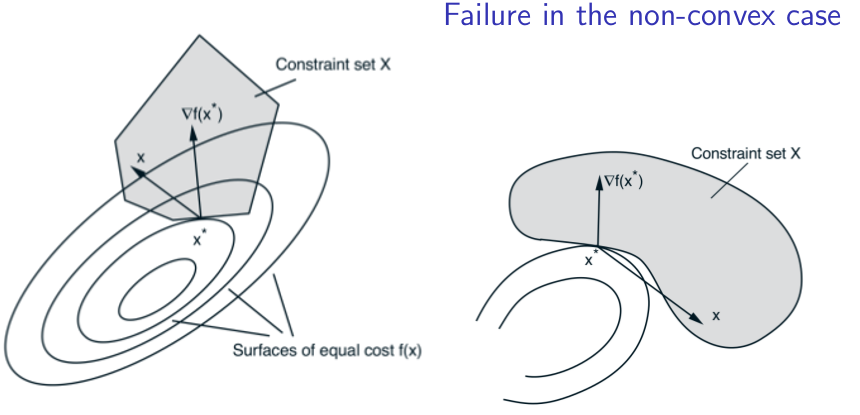
\includegraphics[width=0.8\textwidth]{non_convex.png}
  \caption{Differences between convex and non-convex sets
  \label{fig:non-convex}}
\end{figure}

%%%%%%%%%%%%%%%%%%%%%%%%%%%%%%%%%%%%%%%%%%%%%%%%%%%%%%%%%%%
%25 exact same
\begin{question}
  Explain the projection on a convex set? Write down the projection theorem. Compute the projection of a point $z \in \RR^n$ to the constraint set $C = \{x \in \RR^n:Ax=0\}$
\end{question}

\textbf{\textit{Projection on a convex set:}}
		Let $z$ be a fixed vector in $\RR^n$ and consider finding a vector $x^{*}$ in a closed convex set C, which is at a minimum (squared) distance from $z$
		$$ x^{*} = arg \min_x \frac{1}{2} ||x- z ||^2, \quad s.t. \enspace x \in C$$		
		This problem is called the projection of $z$ on $C$ denoted by $x^{*} = proj_C(z)$ 	
		\begin{figure}[H]
			\centering
			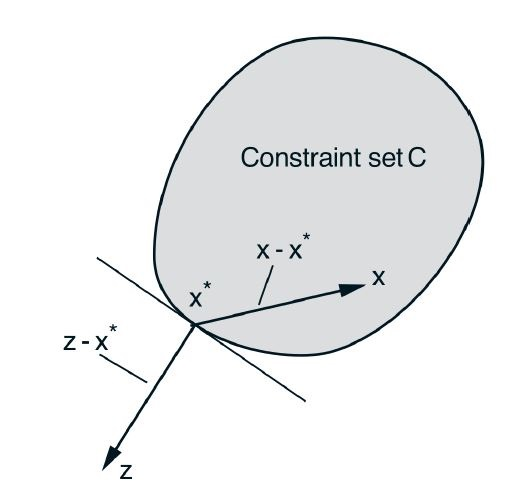
\includegraphics[width=0.5\textwidth]{figures/proj_C.jpg}
		\end{figure}
		
	\textbf{\textit{Projection theorem:}} Let $C$ be a closed and convex set and let $z \in \RR^n$. Then $x^{*}= proj_C(z)$ if and only if
		$$(z-x^{*})^T (y -x^{*}) \le 0, \quad \forall y \in C $$
	
	\textbf{\textit{Compute $z$:}}
	The projection is given by
	\begin{equation*}
	    x^* = proj_C(z)
	\end{equation*}
	Concretely:
	\begin{equation*}
	    x^* = (I - A^T(AA^T)^{-1} A) z
	\end{equation*}


%%%%%%%%%%%%%%%%%%%%%%%%%%%%%%%%%%%%%%%%%%%%%%%%%%%%%%%%%%%
%26 exact same
%%%%%%%%%%%%%%%%%%%%%%%%%%%%%%%%%%%%%%%%%%%%%%%%%%%%%%%%%%% 
\begin{question}
Show that stationarity in optimization over a convex set can also be written in terms of the projection operator.
\end{question}

\textit{Theorem 13} Let f be a continuously differentiable function defined on the closed and convex set
$C$, and let $s > 0$. Then $x^*$ is a stationary point of the problem (P) if and only if
$$x^* = proj_C(x^* - s\nabla f(x^*)).$$

\textit{Proof} From the projection theorem, it follows that 
$x^* = proj_C (\underbrace{x^* - s\nabla f (x^*)}_{z})$ if and only if
$((\underbrace{x^* - s\nabla f (x^*)}_{z}) - x^* )^T (x - x^* ) \leq 0$ for all $x \in C$. This is clearly equivalent to the stationarity condition $\nabla f (x^*)^T (x - x^* ) \geq 0$ (remove the braces around $z$ on the left hand side, cancel out $x^* - x^*$ and multiply by $-1$).
  \begin{flushright}
    $\square$
  \end{flushright}

%%%%%%%%%%%%%%%%%%%%%%%%%%%%%%%%%%%%%%%%%%%%%%%%%%%%%%%%%%%
%27 exact same
%%%%%%%%%%%%%%%%%%%%%%%%%%%%%%%%%%%%%%%%%%%%%%%%%%%%%%%%%%% 
\begin{question}
What is the gradient projection method. Give the algorithm and give choices for the step size selection. Draw an example illustrating the iterations of the gradient projection method.
\end{question}


The gradient projection method takes steps by taking normal descent directions and then projecting them onto the given constraint set $X$ to get feasible descent direction vectors.

\textbf{Iteration:}
\begin{align*}
    \Bar{x}^{(k)} &= {\text{proj}}_{X}(x^{(k)} - s^{(k)} \nabla f(x^{(k)}))\\
    x^{(k+1)} &= x^{(k)} + \alpha^{(k)} (\Bar{x}^{(k)} - x^{(k)})
\end{align*}

For a step size $\alpha \in (0,1]$ and positive scalars $s^{(k)}$.
We take a step in the negative gradient direction (as in steepest descent), and then project it onto $X$ to obtain the feasible vector $\Bar{x}^{(k)}$.

In case of $\alpha^{(k)} = 1$ the method takes the easier form
\begin{equation*}
    x^{(k+1)} = \text{proj}_{X} (x^{(k)} - s^{(k)} \nabla f(x^{(k)})).
\end{equation*}

If $x^{(k)} - s^{(k)} \nabla f(x^{(k)}) \in X$, the projection is trivial and the method reduces to steepest descent. (See Figure \ref{fig:grad_proj_method})

\begin{figure}[H]
    \centering
    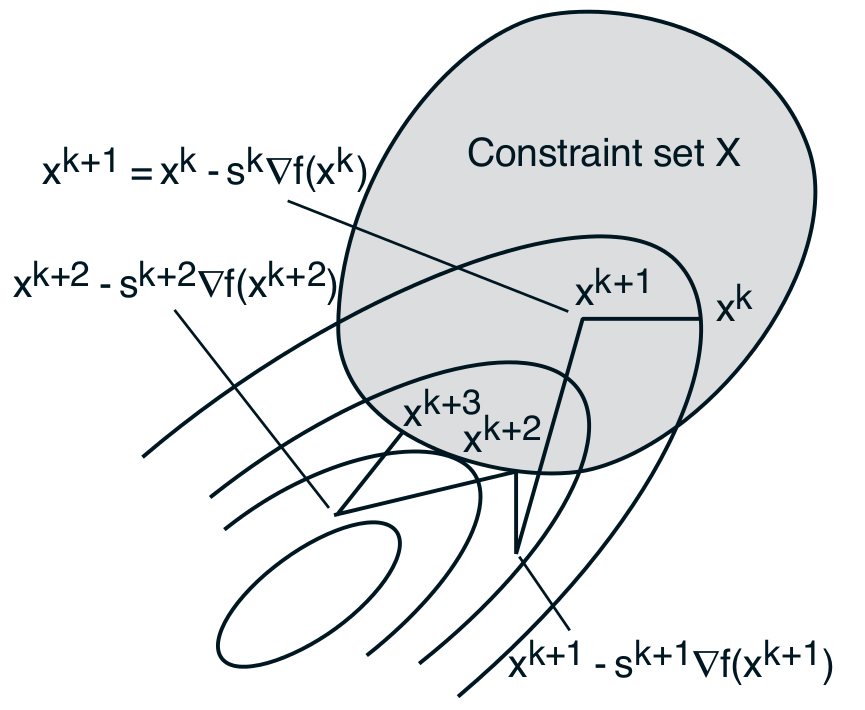
\includegraphics[scale=0.3]{gradient_projection_method}
    \caption{Gradient Projection Method with step size $\alpha^{(k)} = 1$. Inside $X$ the projection is trivial and we only do a normal gradient step.}
    \label{fig:grad_proj_method}
\end{figure}

%%%%%%%%%%%%%%%%%%%%%%%%%%%%%%%%%%%%%%%%%%%%%%%%%%%%%%%%%%%
%28 exact same
%%%%%%%%%%%%%%%%%%%%%%%%%%%%%%%%%%%%%%%%%%%%%%%%%%%%%%%%%%% 
\begin{question}
What is the scaled gradient projection method? Show how to specialize your algorithm such that it becomes a projected Newton algorithm.
\end{question}


	\textbf{\textit{Generalize projection method:}} The gradient projection method can also be written in a different form, which in turn, allows to generalize it to arbitrary metrics.
	\begin{align*}
    \kth[k+1]{x} &= proj_C(\kth{x} - \kth{t} \nabla f(\kth{x}))
    \\ &= arg \min_{x\in C} \frac{1}{2} \norm{x - \kth{x} + \kth{t}\nabla f(\kth{x})}^2
    \\ &= arg \min_{x\in C} \frac{1}{2\kth{t}}\norm{x -\kth{x}+ \kth{t}\nabla f(\kth{x})}^2
    \\ &= arg \min_{x\in C} \nabla \T{f(\kth{x})} (x - \kth{x}) + \frac{1}{2\kth{t}} \norm{x -\kth{x}}^2.
	\end{align*}
In this formulation we can simply replace the squared norm $\norm{x-\kth{x}}^2$ by a weighted squared norm $\norm{x-\kth{x}}^2_{\kth{H}} = \T{(x-\kth{x})} \kth{H}(x-\kth{x})$ where $\kth{H}$ is a symmetric and positive definite matrix. This gives the scaled gradient projection method

\begin{equation*}
    \kth[k+1]{x} = arg \min_{x\in C} \nabla \T{f(\kth{x})} (x -\kth{x}) + \frac{1}{2\kth{t}}\norm{x-\kth{x}}^{2}_{\kth{H}}.
\end{equation*}
Observe that if $f$ is a twice continuously differentiable function over $C$ and $\kth{H} = \nabla^2 f(\kth{x}) $, then we obtain a projected Newton method
\begin{equation*}
    \kth[k+1]{x} = proj^{\nabla^2 f(\kth{x})}_C (\kth{x} - \kth{t}(\nabla^2 f (\kth{x}))^{-1} \nabla f(\kth{x})).
\end{equation*}



%%%%%%%%%%%%%%%%%%%%%%%%%%%%%%%%%%%%%%%%%%%%%%%%%%%%%%%%%%%
%29 Moritz
\begin{question}
  Derive the affine scaling method for solving an equality constrained LP of the form 
  \begin{equation*}
  \min_x c^T x, \quad\text{s.t. } Ax = b, x \geq 0.
    \end{equation*}
  Show how the LP is solved using a scaled gradient projection method. Why can the inequality constraint be skipped? How can the step size be computed?
\end{question}

The affine scaling method is based on the scaled gradient projection method, by which we generate
the steps using
\begin{equation*}
  \kth[k+1]{x} = \argmin_{x \in X} \T{c} (x - \kth{x}) + \frac{1}{2\kth{t}} ||x - \kth{x}||^{2}_{\kth{H}} \text{ s.t. } Ax=b, x \geq 0
\end{equation*}
One important thing to note here is that in the affine scaling method, the sequence of $\kth{x}$ always stays strictly positive and always satisfies $A\kth{x}=b$.
This assumption lets us choose our step size $\kth{t}$ small enough such that $\kth[k+1]{x} > 0$. This will make the algorithm stay in the interior of the constraint set at all times.

This assumption and its consequences allows us to drop the inequality constraint from the sub-problem that we need to solve in each step of the scaled gradient projection method and the problem becomes

\begin{equation*}
  \kth[k+1]{x} = \argmin_{x \in X} \T{c} (x - \kth{x}) + \frac{1}{2\kth{t}} ||x - \kth{x}||^{2}_{\kth{H}} \text{ s.t. } Ax=b
\end{equation*}

Since the problem is linear, we can calculate the exact solution of this quadratic intermediate
problem, and get an update of
\begin{equation}
\label{eq:affine_scaling}
    \kth[k+1]{x} = \kth{x} - \kth{t}(\kth{H})^{-1} (I - \T{A} (A(\kth{H})^{-1} \T{A})^{-1} A (\kth{H})^{-1})c
\end{equation}

Now the step size needs to be selected small enough such that $\kth[k+1]{x} > 0$.
We begin by rewriting the above equation in the gradient descent form
\begin{align}
\kth[k+1]{x} &= \kth{x} + \kth{t} \kth{d}\\
\kth{d} &= -(\kth{H})^{-1} (I-\T{A}(A(\kth{H})^{-1} \T{A})^{-1} A(\kth{H})^{-1})c\\
\kth{t}_{i} &= -\frac{\kth{x}_{i}}{\kth{d}_{i}}\\
\kth{t} &= \alpha \min \{ \kth{t}_{i} : \kth{t}_{i} > 0 \}, \alpha \in (0,1)
\end{align}

\emph{Explanation:}
\begin{enumerate}[(1)]
    \item Begin by rewriting \autoref{eq:affine_scaling} from above in the gradient descent form.
    \item The direction $\kth{d}$ then becomes this.
    \item The element-wise step sizes $\kth{t}_{i}$ are computed such that $\kth[k+1]{x}_{i} = 0$ for all $i = 1 \dots n$.
    \item We can ignore the step sizes where $\kth{d}_{i} > 0$ because otherwise $\kth[k+1]{x}_{i} = \kth{x}_{i} + t \kth{d}_{i} > \kth{x}_{i}$ for some $t > 0$. This gives us the largest possible positive step size in this form. Parameter $\alpha$ ensures the strict positiveness of $\kth[k+1]{x}$.
\end{enumerate}

The metric $\kth{H}$ is chosen by
\begin{equation*}
  \kth{H} = \diag((\kth{x}_1)^{-2}, \dots, (\kth{x}_n)^{-2}).
\end{equation*}

This $\kth{H}$ is the Hessian matrix of the barrier function, i.e. $\kth{H} = \nabla^2 b(\kth{x})$ with
\begin{equation*}
    b(x) = - \sum_{i=1}^n log(x_i)
\end{equation*}

This metric ensures that the algorithm stays inside the boundary of the constraint set $x \geq 0$ by becoming really big at said boundary and therefore "pushing" the gradient away.

Side note: This algorithm uses the inverse $(\kth{H})^{-1}$, but since it is a diagonal matrix it is very easy to invert:
\begin{equation*}
    (\kth{H})^{-1} = \diag((\kth{x}_1)^{2}, \dots, (\kth{x}_n)^{2})
\end{equation*}

%%%%%%%%%%%%%%%%%%%%%%%%%%%%%%%%%%%%%%%%%%%%%%%%%%%%%%%%%%%
% 30 Alice
%%%%%%%%%%%%%%%%%%%%%%%%%%%%%%%%%%%%%%%%%%%%%%%%%%%%%%%%%%% 
\begin{question}
Derive the dual affine scaling method for an inequality constrained LP of the form 
\begin{equation*}
  \max_y b^Ty, \quad\text{s.t. }A^Ty\leq c
\end{equation*}
Derive the scaled gradient projection method and show how the metric is chosen.
\end{question}

We consider a scaled gradient projection method (where we first turn the maximization problem in an equivalent minimization problem)
\begin{equation*}
    \kth[k+1]{y} = \argmin_y -b^T (y - \kth{y}) + \frac{1}{2\kth{t}} \norm{y - \kth{y}}^2_{\kth{H}} \text{ s.t. } A^Ty \leq c
\end{equation*}

where $\kth{H}$ is a metric which still has to be specified. In order to define an appropriate metric, we introduce slack variables $s = c - A^T y$ and note that the linear inequality constraint $A^T y \leq c$ can also be written as $s \geq 0$.
Comparing this expression with the primal affine scaling, we see that a suitable metric that bends the solution away from the boundary would be based on the slack variable $s$ instead of the dual variable y. Let us choose $\kth{H} = A\kth{\tilde{H}}A^T$ , which yields
\begin{equation*}
    \norm{y - \kth{y}}^2_{\kth{H}} = (y - \kth{y})^T \kth{H} (y - \kth{y}) = (y - \kth{y})^T A \kth{\tilde{H}} A^T (y - \kth{y}) = \norm{A^T (y - \kth{y})}^2_{\kth{\tilde{H}}}
\end{equation*}

The important observation is now that $A^T (y-\kth{y}) = \kth{s}-s$ and hence, the obvious choice for the metric $\kth{\tilde{H}}$ is
\begin{equation*}
    \kth{\tilde{H}}=\diag((\kth{s_1})^{-2},(\kth{s_2})^{-2},...,(\kth{s_n})^{-2}).
\end{equation*}
Now, assuming, we have given a strictly feasible point $\kth{s} = c -A^T \kth{y} > 0,$ we can again drop the inequality constraint $s = x -A^T y \geq 0 $and enforce it later during the step size selection.
Hence we are left with solving the simple quadratic problem
\begin{equation*}
    \kth[k+1]{y}=\argmin_y -b^T(y-\kth{y}) + \frac{1}{2\kth{t}}\norm{A^T(y-\kth{y})}_{\kth{\tilde{H}}}^2.
\end{equation*}

Its solution is given by computing the gradient with respect to $y$ and setting it to zero:
\begin{equation*}
    -\kth{t}b + A\kth{\tilde{H}}A^T(y-\kth{y}) = 0.
\end{equation*}
Solving for y yields the iterations of the dual affine scaling method
\begin{equation*}
    \kth[k+1]{y} = \kth{y} + \kth{t}(A\kth{\tilde{H}} A^T)^{-1}b,
\end{equation*}
where the step size $\kth{t}$ must again be chosen small enough such that $\kth[k+1]{s} = \kth{s} - A^T (y^{k+1} - \kth{y}) = \kth{s} - \kth{t} A^T (A \kth{\tilde{H}} A^T)^{-1}b > 0, $ which can be achieved with a similar procedure as described above.

%%%%%%%%%%%%%%%%%%%%%%%%%%%%%%%%%%%%%%%%%%%%%%%%%%%%%%%%%%%
% 31 exact same
\begin{question}
What is the Lagrange multiplier theorem for equality constrained optimization problems? Draw a simple example and explain why the gradients of the constraint functions need to be linearly independent.
\end{question}


We have a problem of the form:
\begin{equation*}
    \underset{x}{\text{min}} f(x) \quad \text{s.t.} \enspace g(x) = c
\end{equation*}
with $g(x)$ being some equality constraint and $c$ being some constant.

The Lagrange multiplier theorem for equality constrained optimization problems tells us that at the optimum of $f$ the following holds:
\begin{equation*}
    \nabla f(x)=\lambda \nabla g(x)
\end{equation*}

Or written as the Lagrange function:
\begin{equation*}
    \mathcal{L}(x, \lambda) = f(x) - \lambda g(x)
\end{equation*}

This means that in the optimum of $f$, the level lines of the function $f$ itself and the constraint function $g$ are tangent which also means that $\nabla f(x)$ and $\nabla g(x)$ are proportional. An example of the tangent level lines can be seen in Figure \ref{fig:lagrange}.

(The Lagrange multiplier $\lambda$ can be either positive or negative depending on the function and the constraints).

For multiple constraints the theorem looks like this:
\begin{equation*}
    \nabla f(x) = \sum_{k=1}^{M} \lambda_k \nabla g_k (x)
\end{equation*}
Now we have multiple Lagrange multipliers $\lambda_1, \dots , \lambda_M$.

\textbf{Linear independence of the gradients of the constraint functions:}\\
At the optimal value, the gradient of the cost function $f$ lies in the subspace spanned by the gradients of the constraint functions $g_k$. For those functions to span a subspace, they need to be linearly independent.

\begin{figure}
    \centering
    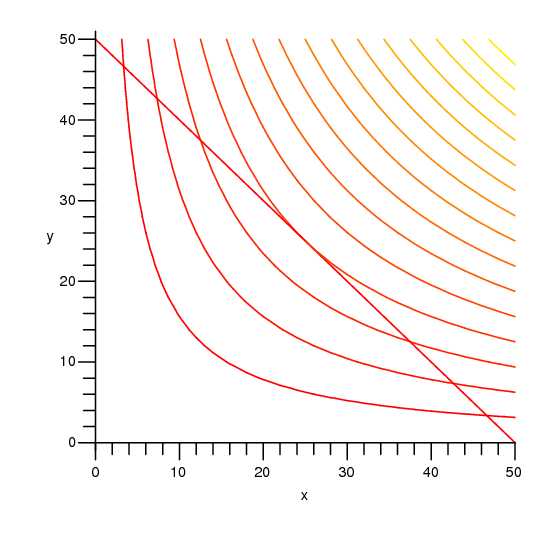
\includegraphics[scale=0.5]{figures/lagrange.png}
    \caption{Example for the Lagrange multiplier theorem. Here we see that the level lines of the function and the constraint function are tangent.}
    \label{fig:lagrange}
\end{figure}

%%%%%%%%%%%%%%%%%%%%%%%%%%%%%%%%%%%%%%%%%%%%%%%%%%%%%%%%%%%

\end{document}
